\documentclass[10pt]{beamer}

\usetheme{metropolis}
\usepackage{appendixnumberbeamer}

\usepackage{outlines}

\title{RUNTIME ADAPTIVE REDUCTION OF TASK OVERHEADS IN HPX}
\subtitle{General Exam Presentation}
\author{Bibek Wagle}
\date{May 2, 2018}
\institute{Division of Computer Science and Engineering \\ School of Electrical Engineering and Computer Science \\ Louisiana State University}
\titlegraphic{
\includegraphics[height=10mm]{logos/stellar_4x1.pdf}}
\titlegraphic{
	\begin{tikzpicture}[overlay, remember picture]
	\node[at=(current page.south east), anchor=south east] {%
		
\includegraphics[width=.25\textwidth]{logos/stellar_4x1.pdf} 
	};
	\node[at=(current page.south west), anchor=south west] {%
		
\includegraphics[width=.50\textwidth]{logos/cct_logo.pdf} 
	};
	\end{tikzpicture}
}


\begin{document}
\setbeamercolor{background canvas}{bg=white}
\maketitle

\begin{frame}{Outline}
  \setbeamertemplate{section in toc}[sections]
  \tableofcontents[hideallsubsections]
\end{frame}

\section{Introduction}

\begin{frame}{High Performance Computing Today}
\begin{outline}
	\1 Size of clusters are increasing rapidly
		\2 \alert{Tianhe-2} has 16,000 compute nodes with a total of 3,120,000 cores
		\2 \alert{Sunway TiahuLight} has 40,906 compute nodes with a total of 10,649,600 cores
	\1 Each node with many cores rather than a powerful single core
	\1 \alert{How do we make efficient use of such abundant processing power ?}
\end{outline}
\end{frame}

\begin{frame}{Software Stack for the HPC}
\begin{outline}
	\1 MPI is the de facto standard for HPC
	\1 Long history, designed in the 90s
	\1 MPI + X is largely used 
	\1 X = OpenMP, Pthreads, C++ Threads
\end{outline}
\end{frame}

\begin{frame}{Task Based Runtime Systems}
\begin{outline}
	\1 Replacement for the MPI + X Model 
	\1 Based on decomposing algorithms into fine grained unit of work(tasks)
	\1 Asynchronous execution of tasks
	\1 Promise of making full use of the underlying machine
\end{outline}
\end{frame}

\begin{frame}{Runtime Overheads}
\begin{outline}
	\1 Overheads limits runtime system performance  
	\1 One of the key pitfalls of task based runtime systems
	\1 Overheads associated with locally executed tasks
	\1 Overheads associated with distributed task execution
	\1 \alert{Overhead is defined as excess work that needs to be carried out in order to perform actual computation}
\end{outline}
\end{frame}

\begin{frame}{}
\alert{How do we minimize the effect of these overheads?}
\end{frame}

\begin{frame}{Motivation}
\begin{outline}
	\1 Computing trends are shifting towards many core systems which presents more opportunity for high concurrency
	\1 Reducing overheads improves concurrency 
	\1 Overall improvement in application performance
	\1 Reduction in energy consumption
\end{outline}
\end{frame}
%

\section{Managing Network Overhead}

\begin{frame}{Fine Grained Tasks}
\begin{outline}
	\1 Fine grained tasks results in fine grained communication pattern 
	\1 Efficient communication 
		\2 Latency
		\2 Bandwidth
		\2 Overheads associated with creating and sending messages
	\1 What can be done ?
		\2 Efficient use of bandwidth
		\2 \alert{Reduction of overheads}
\end{outline}	
\end{frame}

\begin{frame}{Message Coalescing to Reduce Overheads}
\begin{outline}
	\1 \alert{Message coalescing} is a technique that is useful for reducing overheads
	\1 Combine small messages into large ones
	\1 Effectively send the same amount of data while reducing per message overheads
	\1 Larger messages equates to better bandwidth utilization
\end{outline}
\end{frame}

\begin{frame}{Approaches to Coalescing}
\begin{outline}
	\1 Manual coalescing
		\2 High effort
		\2 Impractical for larger projects
	\1 Runtime system provided coalescing
		\2 HPX, AM++ / Active Pebbles, Charm++
	\1 Issues: 
		\2 How many messages to coalesce?	
		\2 Do different applications need different parameters?
		\2 How do you determine the coalescing parameters?
	\1 Solution: \alert{Intelligent Adaptive coalescing approach that dynamically varies its parameters depending upon application behavior.} 
\end{outline}
\end{frame}

\begin{frame}{Existing Solution for Adaptive Coalescing}
\begin{outline}
	\1 Charm++ exhibits basic adaptive approach for message coalescing
	\1 Application is run automatically with different coalescing parameters each iteration
	\1 Possible improvements:
	\2 Monitor real time network overheads and select coalescing parameters based on this information
	\2 Allow for varying coalescing parameters mid iteration based on the phase of the application
	\2 General adaptive framework that does not require iterative steps or predictable pattern of communication
\end{outline}
\end{frame}

\begin{frame}{Towards Advanced Message Coalescing}
\begin{outline}
	\1 For Advanced general adaptive coalescing framework :
		\2 Implement message coalescing in HPX
		\2 Identification of metrics and runtime characteristics pertaining to fine grained communication overheads
		\2 Utilization of identified metrics and runtime characteristics for adaptive tuning of coalescing parameters.
	\1 Current State:
		\2 Implement message coalescing in HPX : \alert{COMPLETED}
		\2 Identification of metrics and runtime characteristics pertaining to fine grained communication overheads : \alert{COMPLETED}
		\2 Utilization of identified metrics and runtime characteristics for adaptive tuning of coalescing parameters : \alert{IN PROGRESS}
\end{outline}
\end{frame}

\begin{frame}{The HPX Runtime System}
\begin{outline}
	\1 Asynchronous Task based distributed runtime system written mostly in C++
	\1 HPX application can run on both a single machine as well as a cluster with thousands of nodes
	\1 Exposes a concurrency and parallelism API consistent with the ISO C++ standard
	\1 Real time performance measurement capabilities
	\1 Runtime adaptive capabilities
\end{outline}
\end{frame}

\begin{frame}
\begin{figure}
	\centering
	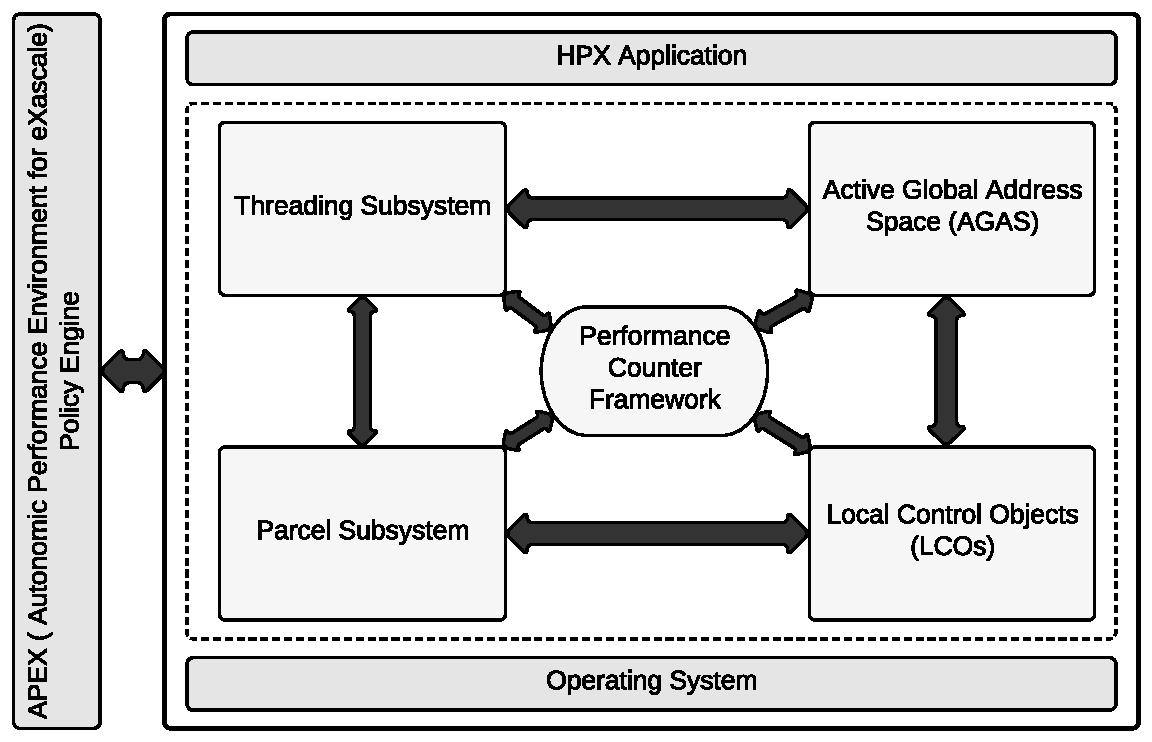
\includegraphics[width=0.72\linewidth]{figures/hpx_arch.pdf}
	\caption{Architecture of HPX}
\end{figure}
The HPX architecture consisting of \alert{AGAS} for addressing any HPX object globally , \alert{LCOs} for synchronization of tasks , \alert{Threading Subsystem} for employing lightweight tasks on OS threads , \alert{Parcel Subsystem for executing tasks remotely}, \alert{Performance counter} framework for instrumentation and debugging purpose and \alert{APEX} for runtime adaptive capabilities. 

\end{frame}

\begin{frame}{The HPX Parcel}
\begin{outline}
	\1 A form of \alert{active message.}
	\1 Created when a method, called \alert{action} in HPX terminology is called remotely 
	\1 Goes though serialization process which converts it into stream of bytes and is sent over the wire
	\1 HPX presently supports : TCP/IP, MPI and IB-Verbs protocols for remote sends
	\1 Reconstructed at the receiving end and placed in scheduler queue for execution
\end{outline}
\begin{figure}
\centering
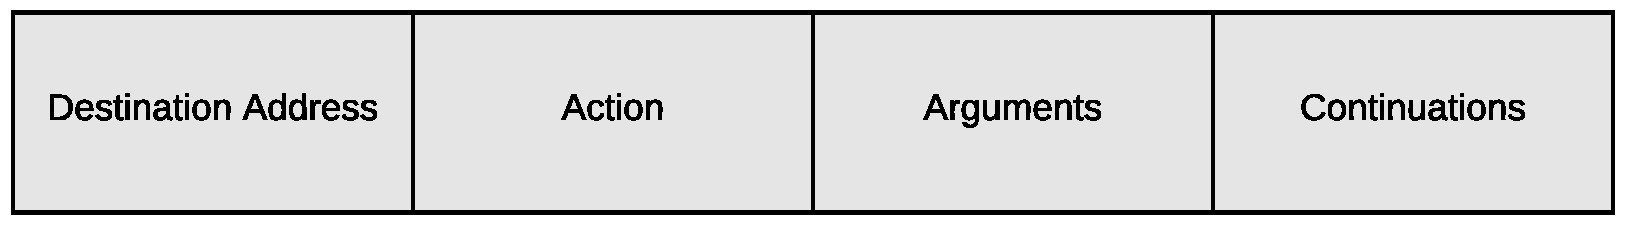
\includegraphics[width=1\linewidth]{figures/hpx_parcel.pdf}
\caption{Structure of a HPX Parcel. A parcel has four components: the destination address; the action, which is the method/function to execute at the destination; the arguments for the function; and optional continuations. }
\end{figure}
\end{frame}

\begin{frame}{Parcel Coalescing}
\begin{figure}
	\centering
	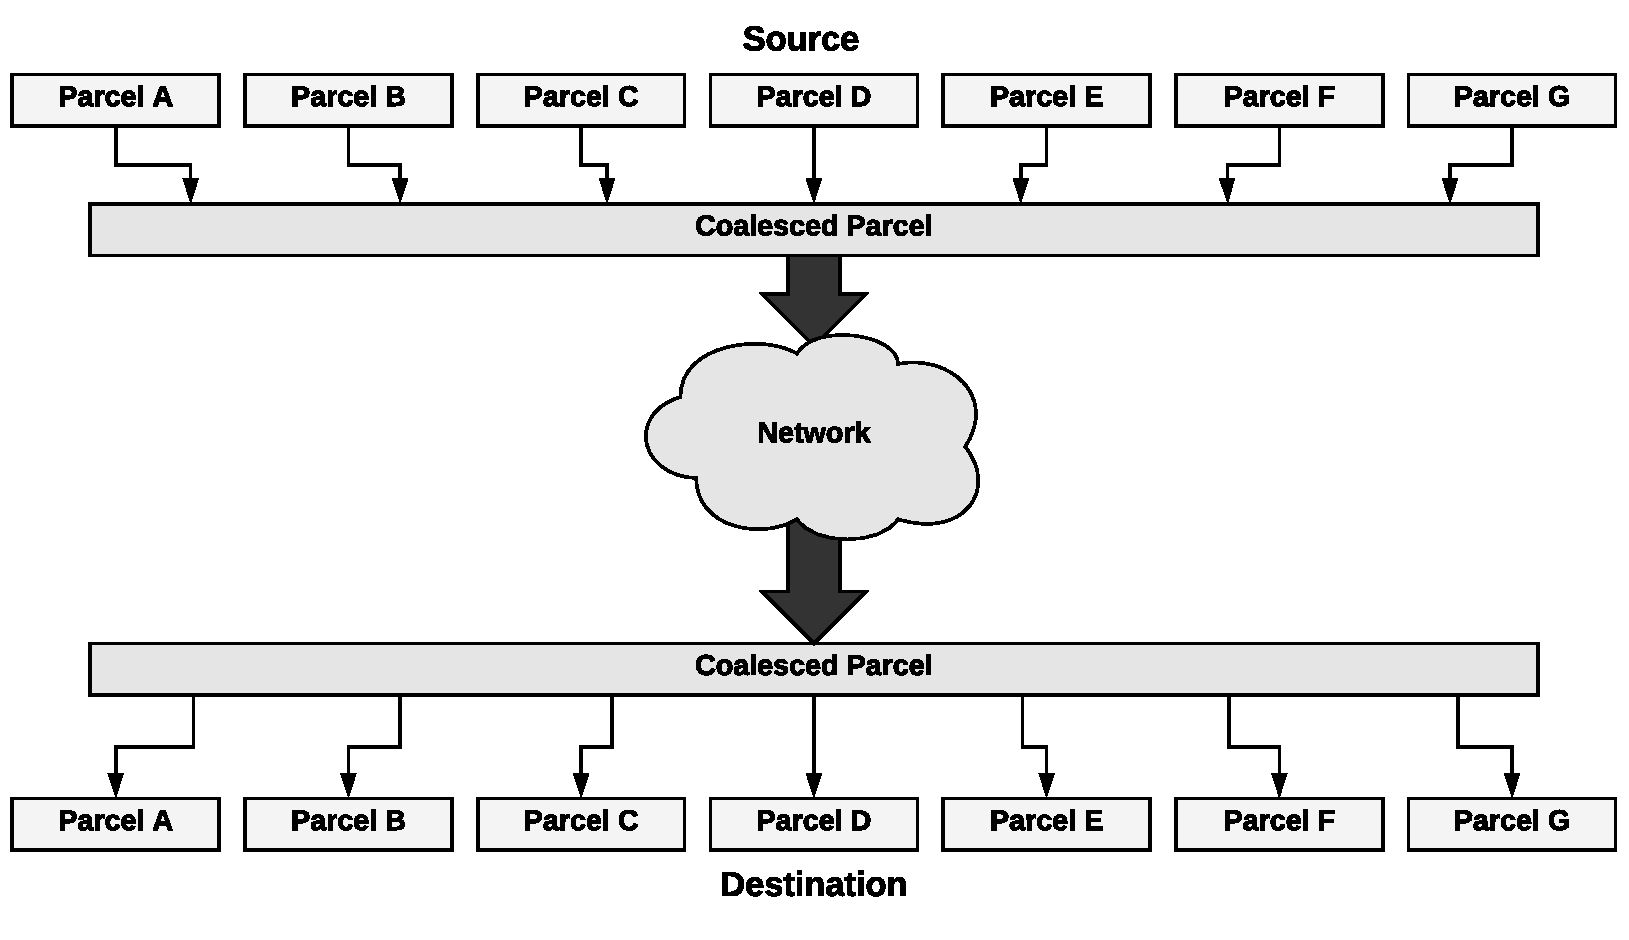
\includegraphics[width=0.8\linewidth]{figures/ParcelCoalescingDiagram.pdf}
	\caption{{A diagrammatic representation of message coalescing. Individual active messages are grouped together to form a large message at the sending end which is reconstructed into the original individual entities at the receiving end.}}
	\label{figureCOAL}
\end{figure}
\end{frame}

\begin{frame}{Parcel Coalescing in HPX}
\begin{outline}
	\1 Designed around two parameters
		\2 Queue length : the number of parcels to coalesce in a single send
		\2 Wait time : time to wait in microseconds for the queue to be full before flushing the queue
	\1 Wait time helps avoid deadlocks 
	\1 Future Work: Use buffer size rather than number of parcels
\end{outline}
\end{frame}

\begin{frame}{Parcel Coalescing in HPX}
\begin{figure}
	\centering
	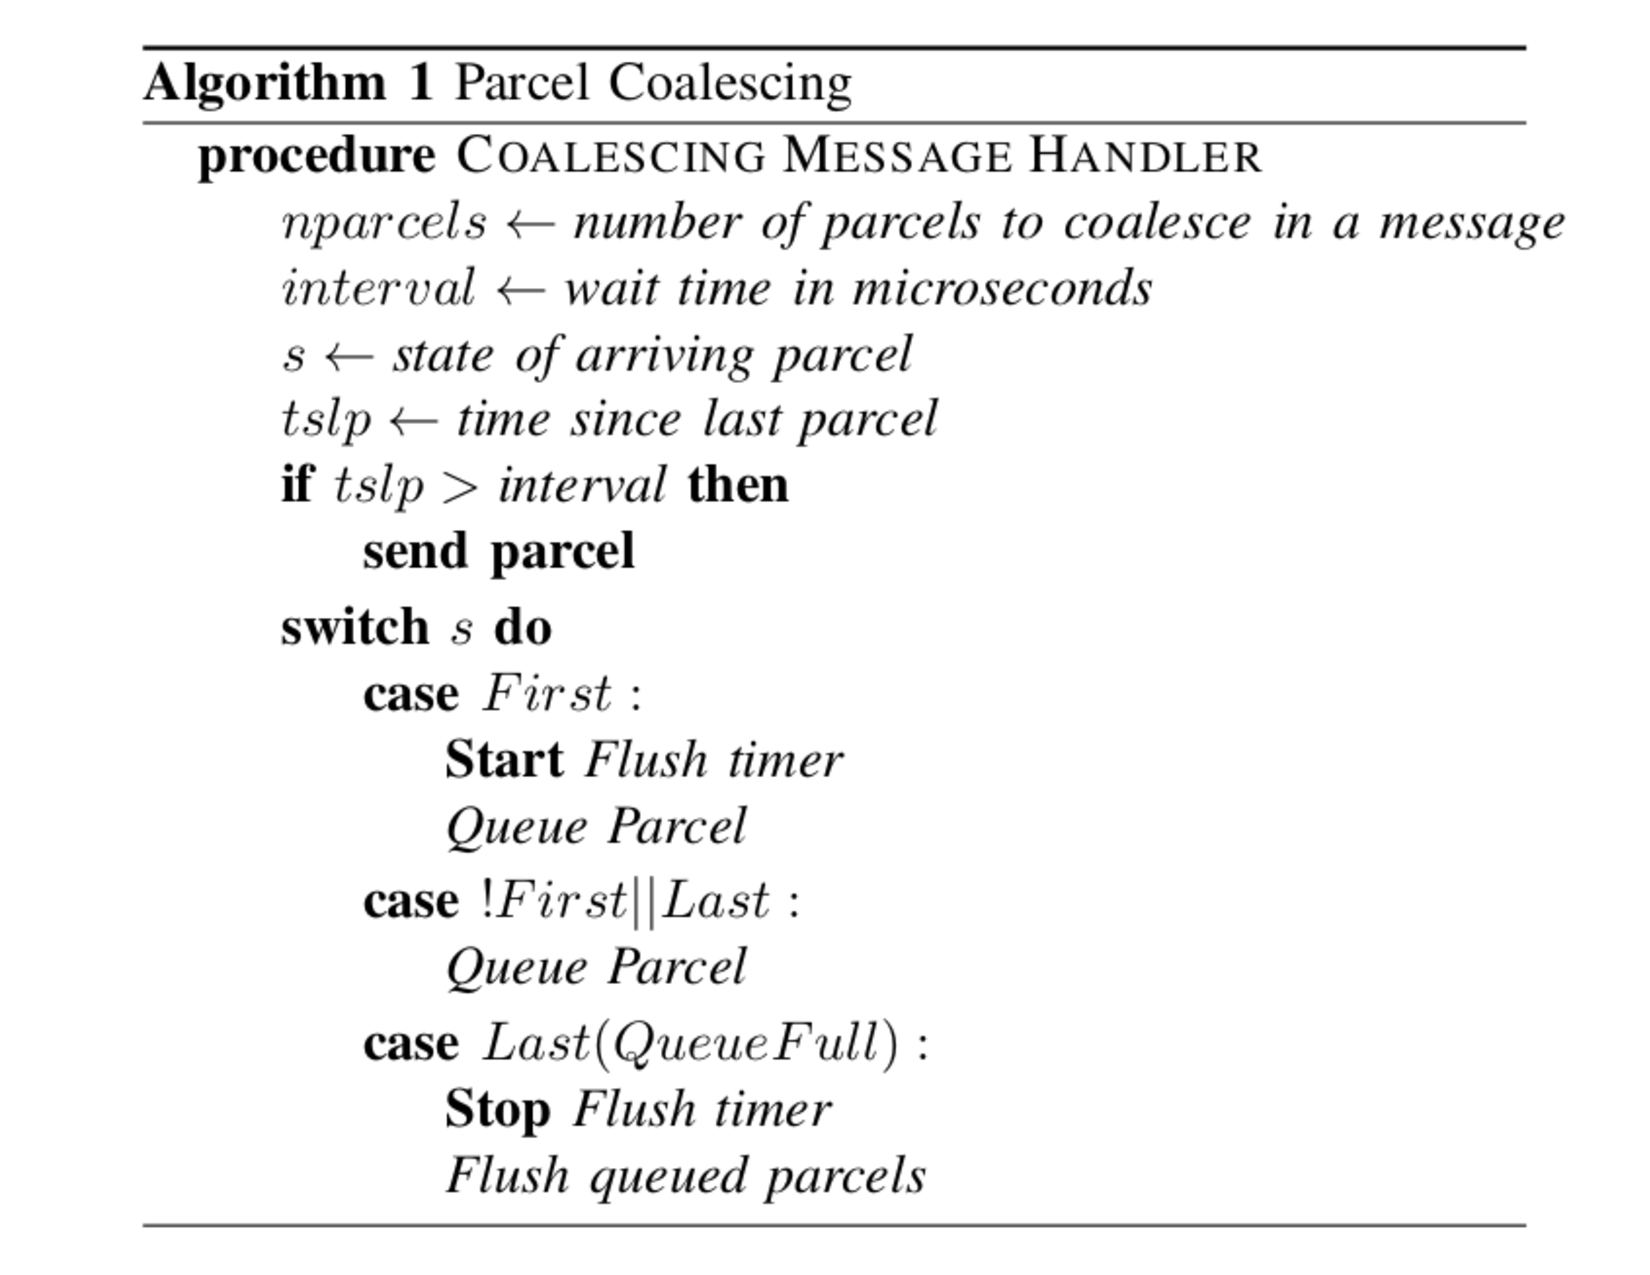
\includegraphics[width=0.8\linewidth]{figures/coalescing_algo.pdf}
	\caption{{Algorithm for HPX implementation of Parcel Coalescing}}
\end{figure}
\end{frame}

\begin{frame}{Network Performance Metrics}
\begin{outline}
	\1 Metrics for measuring network overhead are necessary for achieving our goal of adaptive message coalescing.
	\1 We define overhead as the time spent processing information to be communicated across the network.
\end{outline}
\end{frame}

\begin{frame}{Task Duration}
We looked at the overall time spent on executing each HPX-thread or tasks including the overhead. We define task duration using the following equation:
%
\begin{equation}
t_{d} = \sum{t_{func}}
\label{equ:taskdur}
\end{equation}

where $\sum{t_{func}}$ is the total time spent by the HPX scheduler executing each HPX thread.
\end{frame}

\begin{frame}{Task Overhead}
We then looked at the average time spent on thread management for each HPX-thread or tasks. All communication in HPX is done via tasks. We calculate task overhead using the following equation:
%
\begin{equation}
t_{o} = \frac{\sum{t_{func}}-\sum{t_{exec}}}{n_t}
\label{equ:taskoverhead}
\end{equation}
where ${\sum{t_{exec}}}$ is the time spend by the HPX scheduler doing useful work and  ${\sum{t_{func}}}$ is the task duration as defined in Equation~\ref{equ:taskdur} and ${n_t}$ is the number of executed HPX threads.

\end{frame}

\begin{frame}{Observations}
\begin{outline}
	\1 We observed a positive correlation between task overhead and overall execution time of our test applications for various coalescing parameters.
	\1 After establishing that task overhead has a positive correlation with the overall execution time, we separated the network related overhead from other overheads.
	\1 HPX performs network related tasks such as packaging a parcel into a message, serialization, handshaking and locality resolution in the form of background work.
\end{outline}
\end{frame}

\begin{frame}{Background Work Duration}
 We define total time spent doing background work as the background work duration and it is obtained using the following equation:
\begin{equation}
t_{bd} = \sum{t_{{background-work}}}
\label{equ:bgdur}
\end{equation}
Background Work Duration can be queried using the performance counter \alert{/threads/background-work}.
\end{frame}

\begin{frame}{Network Overhead}
The network overhead count is the ratio of 
thread background work duration to task duration.
Network Overhead is shown in Eq.~\ref{equ:network-oh}.
%
\begin{equation}
n_{oh} = \frac{\sum{t_{{background-work}}}}{\sum{t_{{func}}}}
\label{equ:network-oh}
\end{equation}
%
Here, $\sum{t_{{background-work}}}$ is the total time spent performing network related work and $\sum{t_{{func}}}$ is the total time to reach the completion of each HPX thread.

Hence, Network Overhead gives us the fraction of overall time spent on performing network related work.

The network overhead performance counter can be queried using \alert{/threads/background-overhead} . 
\end{frame}

\begin{frame}{Testing the Network Overhead Metric}
\begin{outline}
	\1 We test for correlation between our Network Overhead metric and overall execution time of our test applications.
	\1 Experimental Testbed 
		\2 Marvin Thin Compute Nodes of ROSTAM Cluster 
		\2 2x Intel Xeon E5-2450 CPU 16 Cores total 
		\2 48GB 1333 MHZ DDR3 Memory 
		\2 HPX v 1.0 , GCC 6.3 , IMPI 2017.2.174
	
\end{outline}
\end{frame}

\begin{frame}{Testing the Network Overhead Metric}
\begin{outline}
	\1 We use two test applications:
		\2 The Parquet Application
		\2 A Toy Example
\end{outline}
\end{frame}

\begin{frame}{The Parquet Application}
\begin{outline}
		\1 A complex physics simulation
		\1 Requires use of many rank-three tensors
		\1 The linear dimension ($N_c$)  of the simulation controls the tensor size
		\1 Throughout the simulation, large number of messages are sent between nodes
		\1 The \alert{rotation phase }sends $8*N_c^2$ parcels containing $N_c$ elements

\end{outline}
\end{frame}

\begin{frame}{Toy Application Example}
\begin{figure}
	\centering
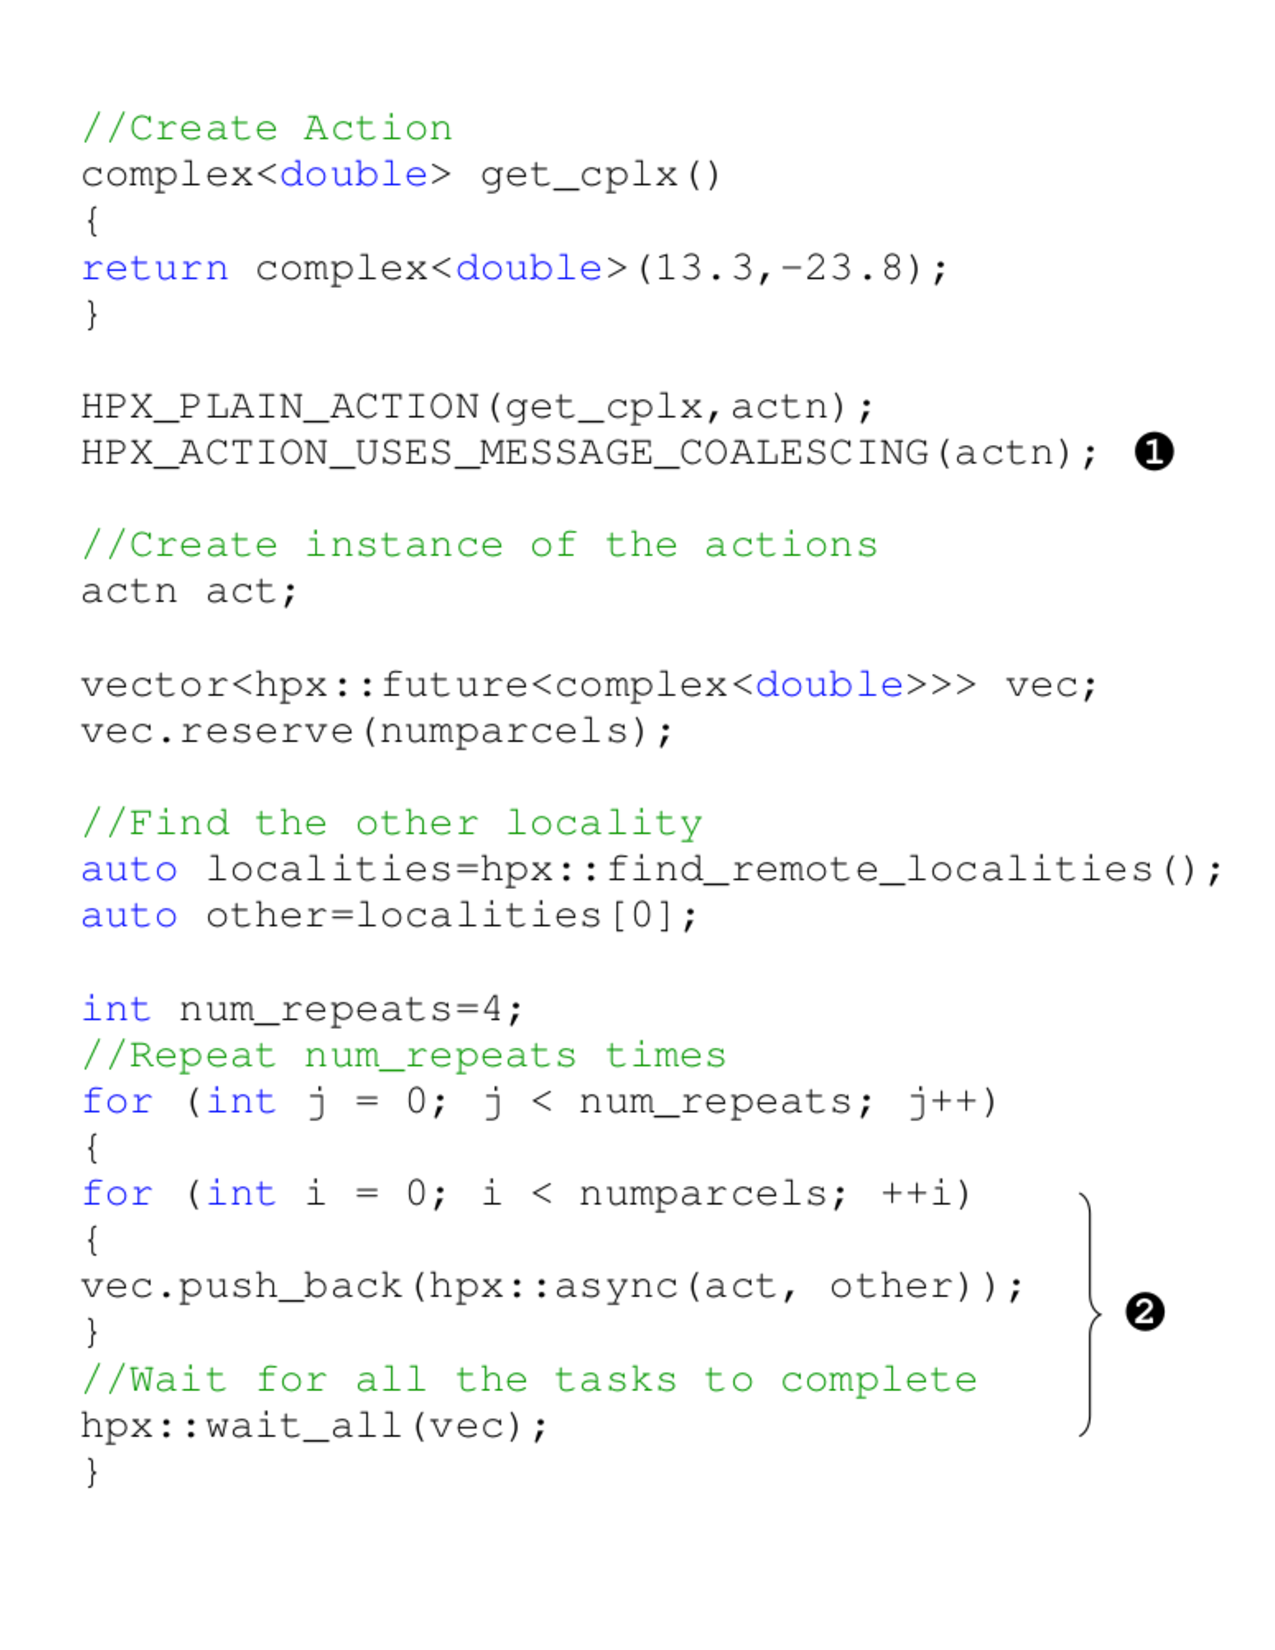
\includegraphics[width=0.52\linewidth]{figures/toy_app_listing.pdf}
\caption{{Toy Application}}
\label{toy_app}
\end{figure}
\end{frame}

\begin{frame}{Definition}
Experiments on the Toy application was performed on two Nodes where each node sent a million messages to each other.\\
We define the process of sending a million message as a phase as shown in annotation 2 in Figure~\ref{toy_app}.
\end{frame}

\begin{frame}{Toy Application Execution Time Per Phase}
\begin{figure}
	\centering
	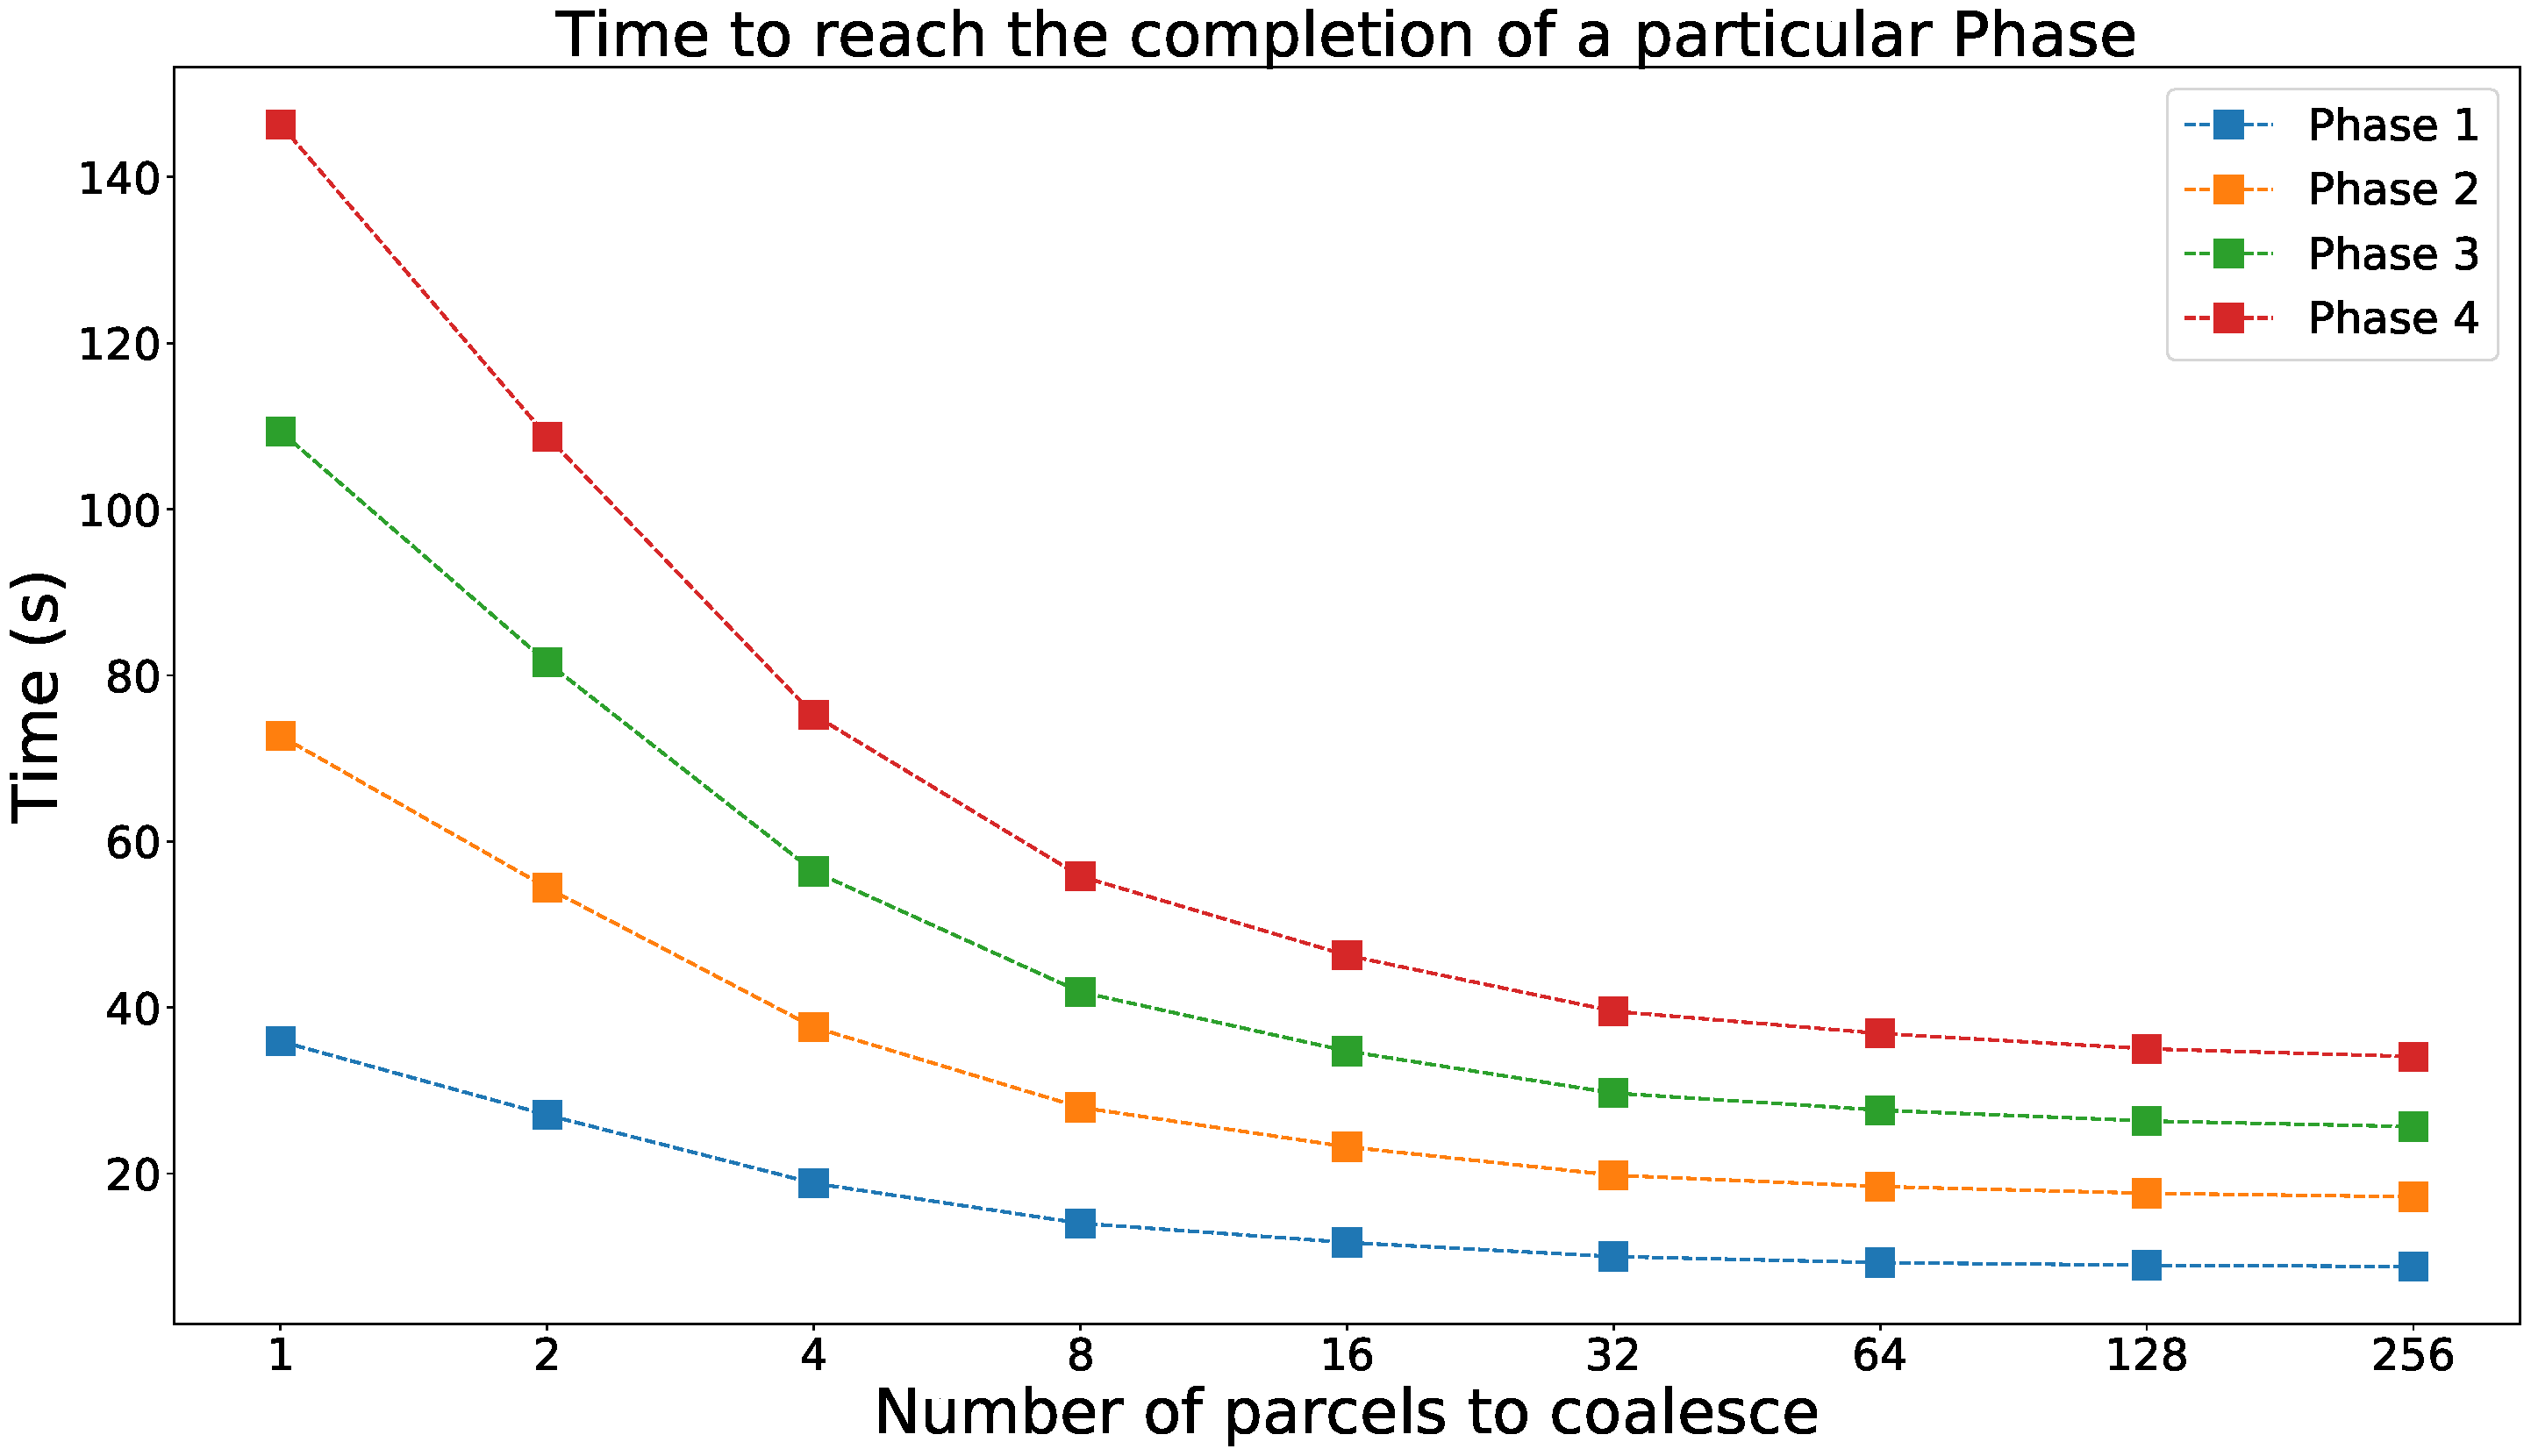
\includegraphics[width=0.8\linewidth]{figures/ToyTimeToReachPhase.pdf}
	\caption{{Time to reach the completion of a particular phase in the toy application for various values of number of parcels to coalesce in a single message with a wait time of 4000$\mu$s. In this example, as more parcels are coalesced, the time to reach the completion of a phase decreases.}}
	\label{figureToyETOHNM}
\end{figure}
\end{frame}

\begin{frame}{Toy Application Network Overhead vs Time Per Phase}
\begin{figure}
	\centering
	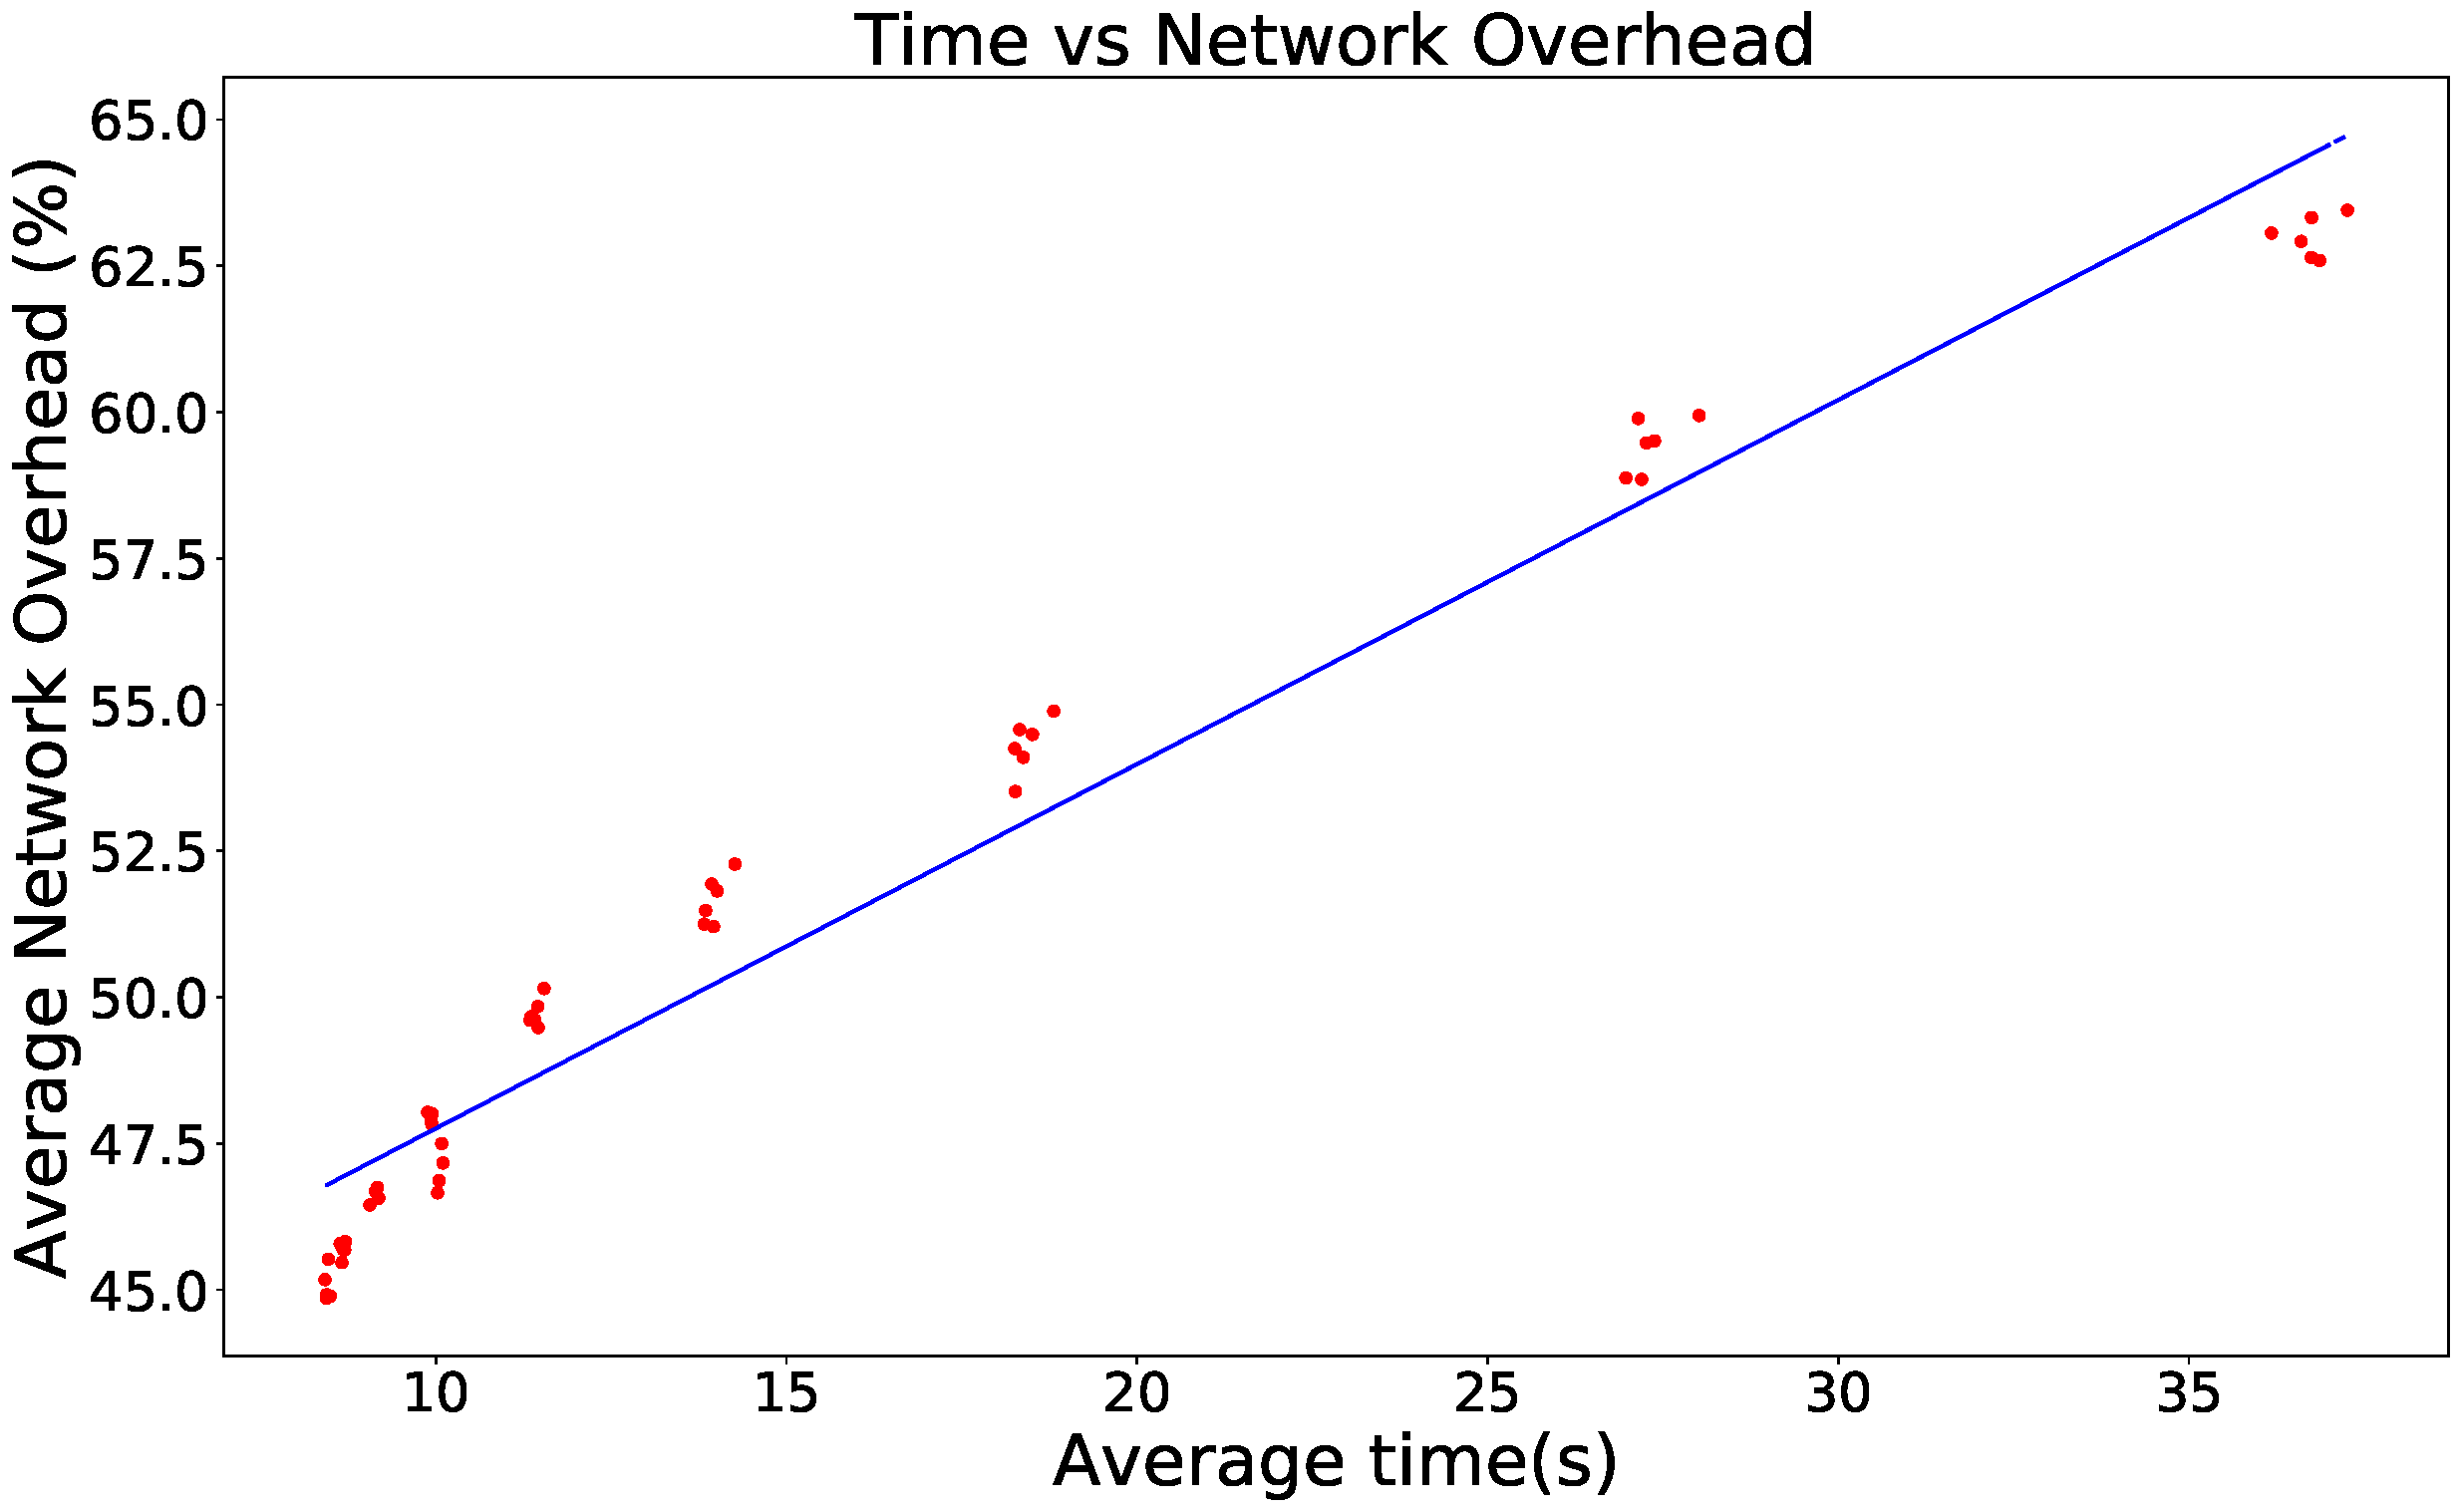
\includegraphics[width=0.8\linewidth]{figures/TimevsOhToyTREND.pdf}
	\caption{{Scatter Plot of the average network overhead per phase vs average execution time per phase for the toy application. Each dot represents a set of parcel coalescing parameters. Average overhead is the average for four phases.  A Pearson's correlation coefficient of 0.97 indicates a strong positive correlation between network overhead and runtime. }}
	\label{figureETVSOH}
\end{figure}
\end{frame}

\begin{frame}{Observations}
\begin{outline}
	\1 Fastest time per iteration seen with largest value of number of parcels to coalesce 
	\2 Lack of dependency with any other communication or computation
	\1 Does not reflect the behavior of a real application
\end{outline}
\end{frame}

\begin{frame}{Parquet Time to Reach a Particular Iteration}
\begin{figure}
	\centering
	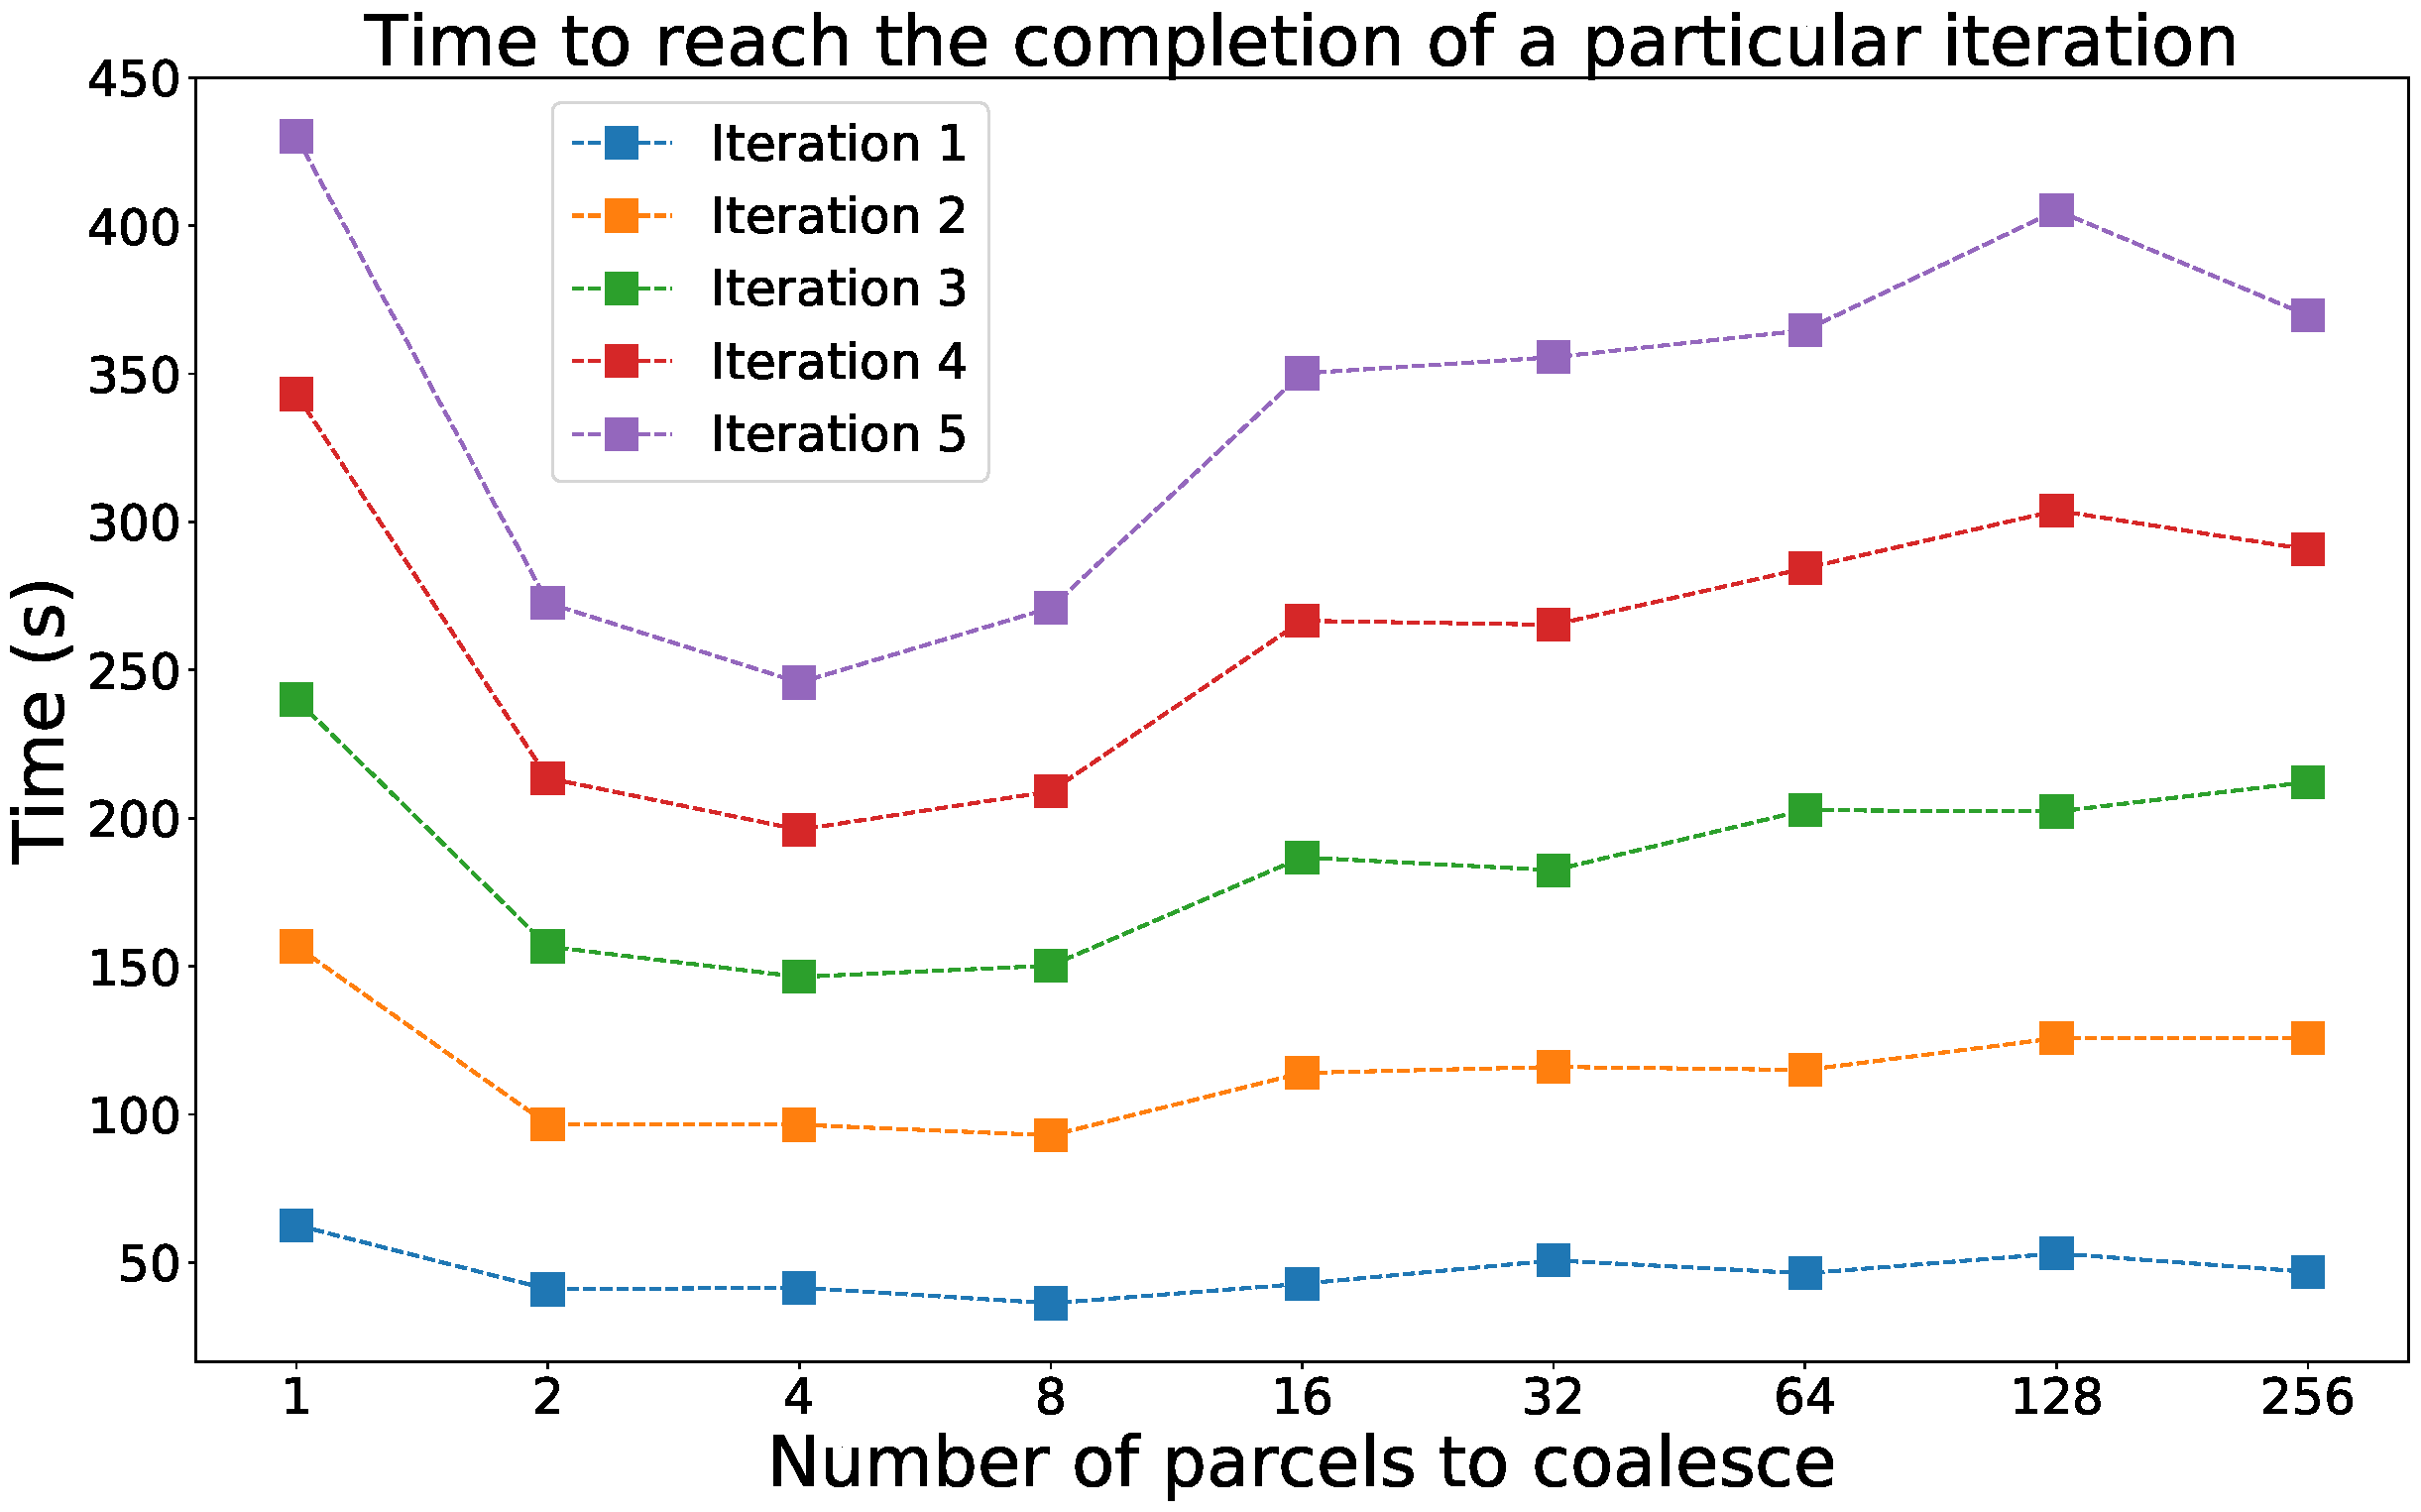
\includegraphics[width=0.8\linewidth]{figures/ParquetTimeToReachIter.pdf}
	\caption{{Time to reach the completion of different iterations in the parquet application for various numbers of parcels coalesced in a single message with a wait time of 4000$\mu$s. Each color indicates a different iteration.}}
	\label{figureTub}
\end{figure}
\end{frame}

\begin{frame}{Parquet Execution Time vs Network Overhead}
\begin{figure}
	\centering
	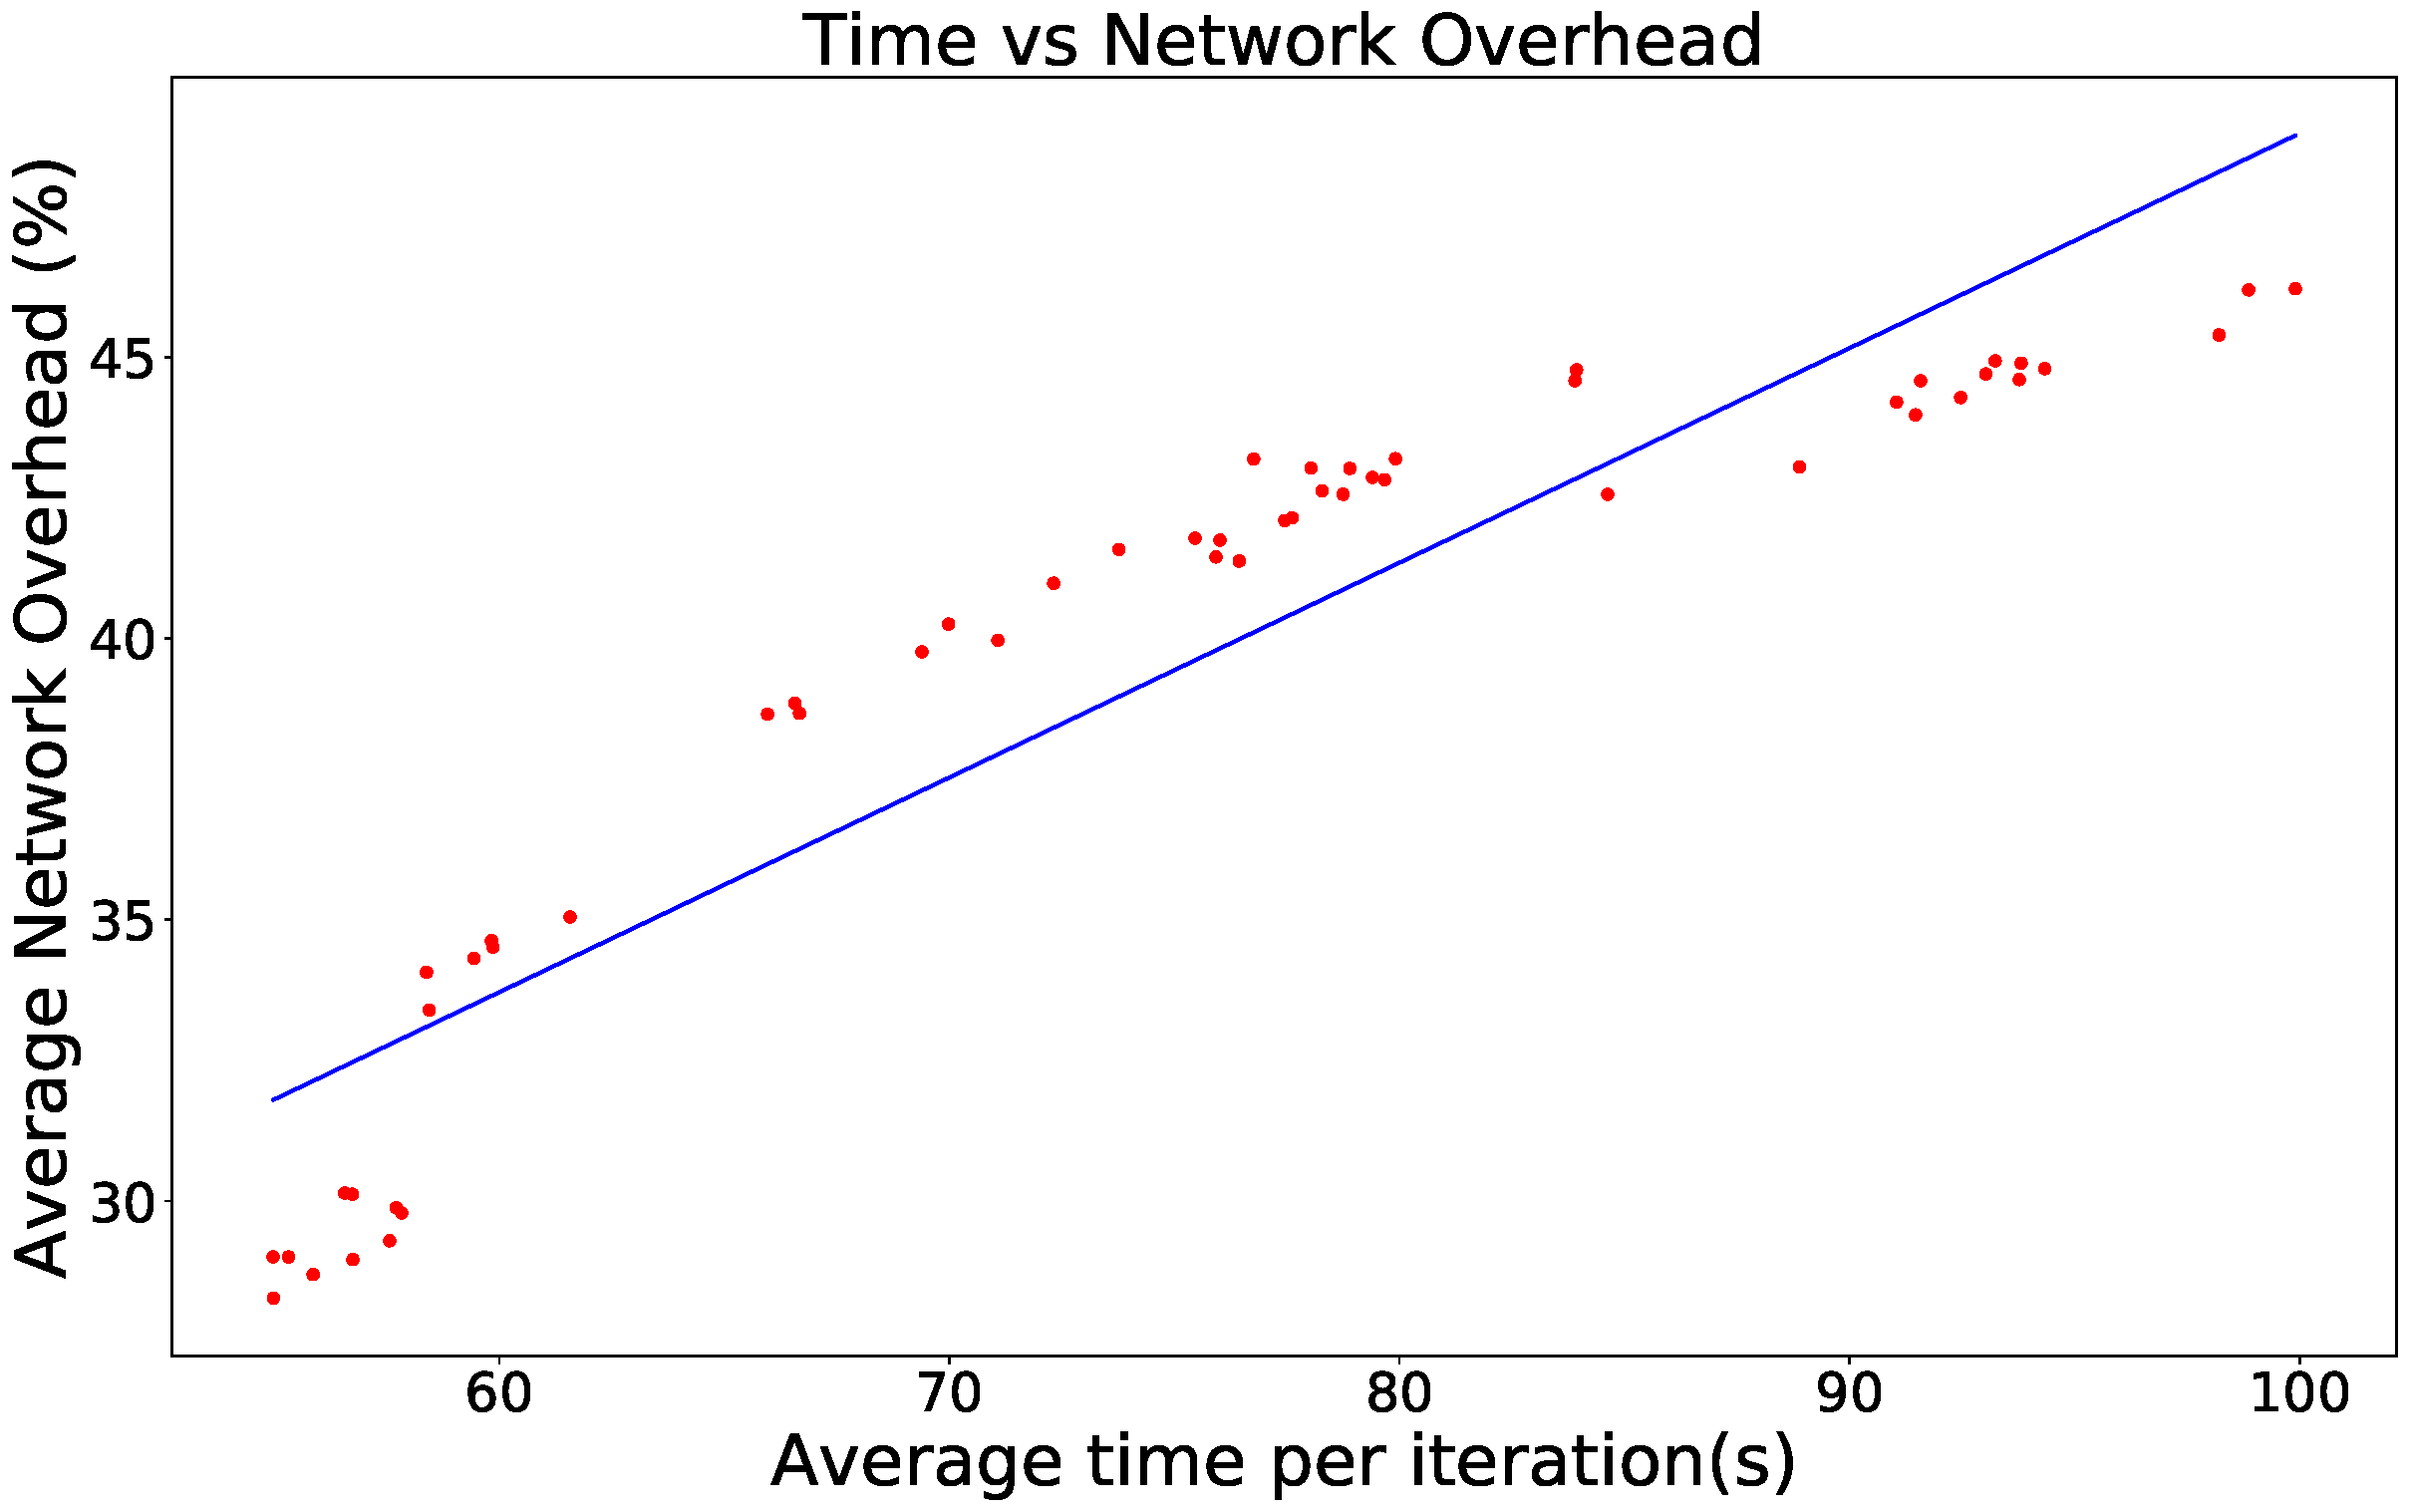
\includegraphics[width=0.8\linewidth]{figures/TimevsOhParquetTREND.pdf}
	\caption{{Scatter Plot of Average Network Overhead Vs Average time per iteration for the Parquet Application. Each dot represents a set of parcel coalescing parameters. A Pearson's correlation coefficient of 0.92 was calculated indicating a strong positive correlation.}}
	\label{figureETVSOHParq}
\end{figure}
\end{frame}

\begin{frame}{Parquet Execution Time}
\begin{figure}
	\centering
	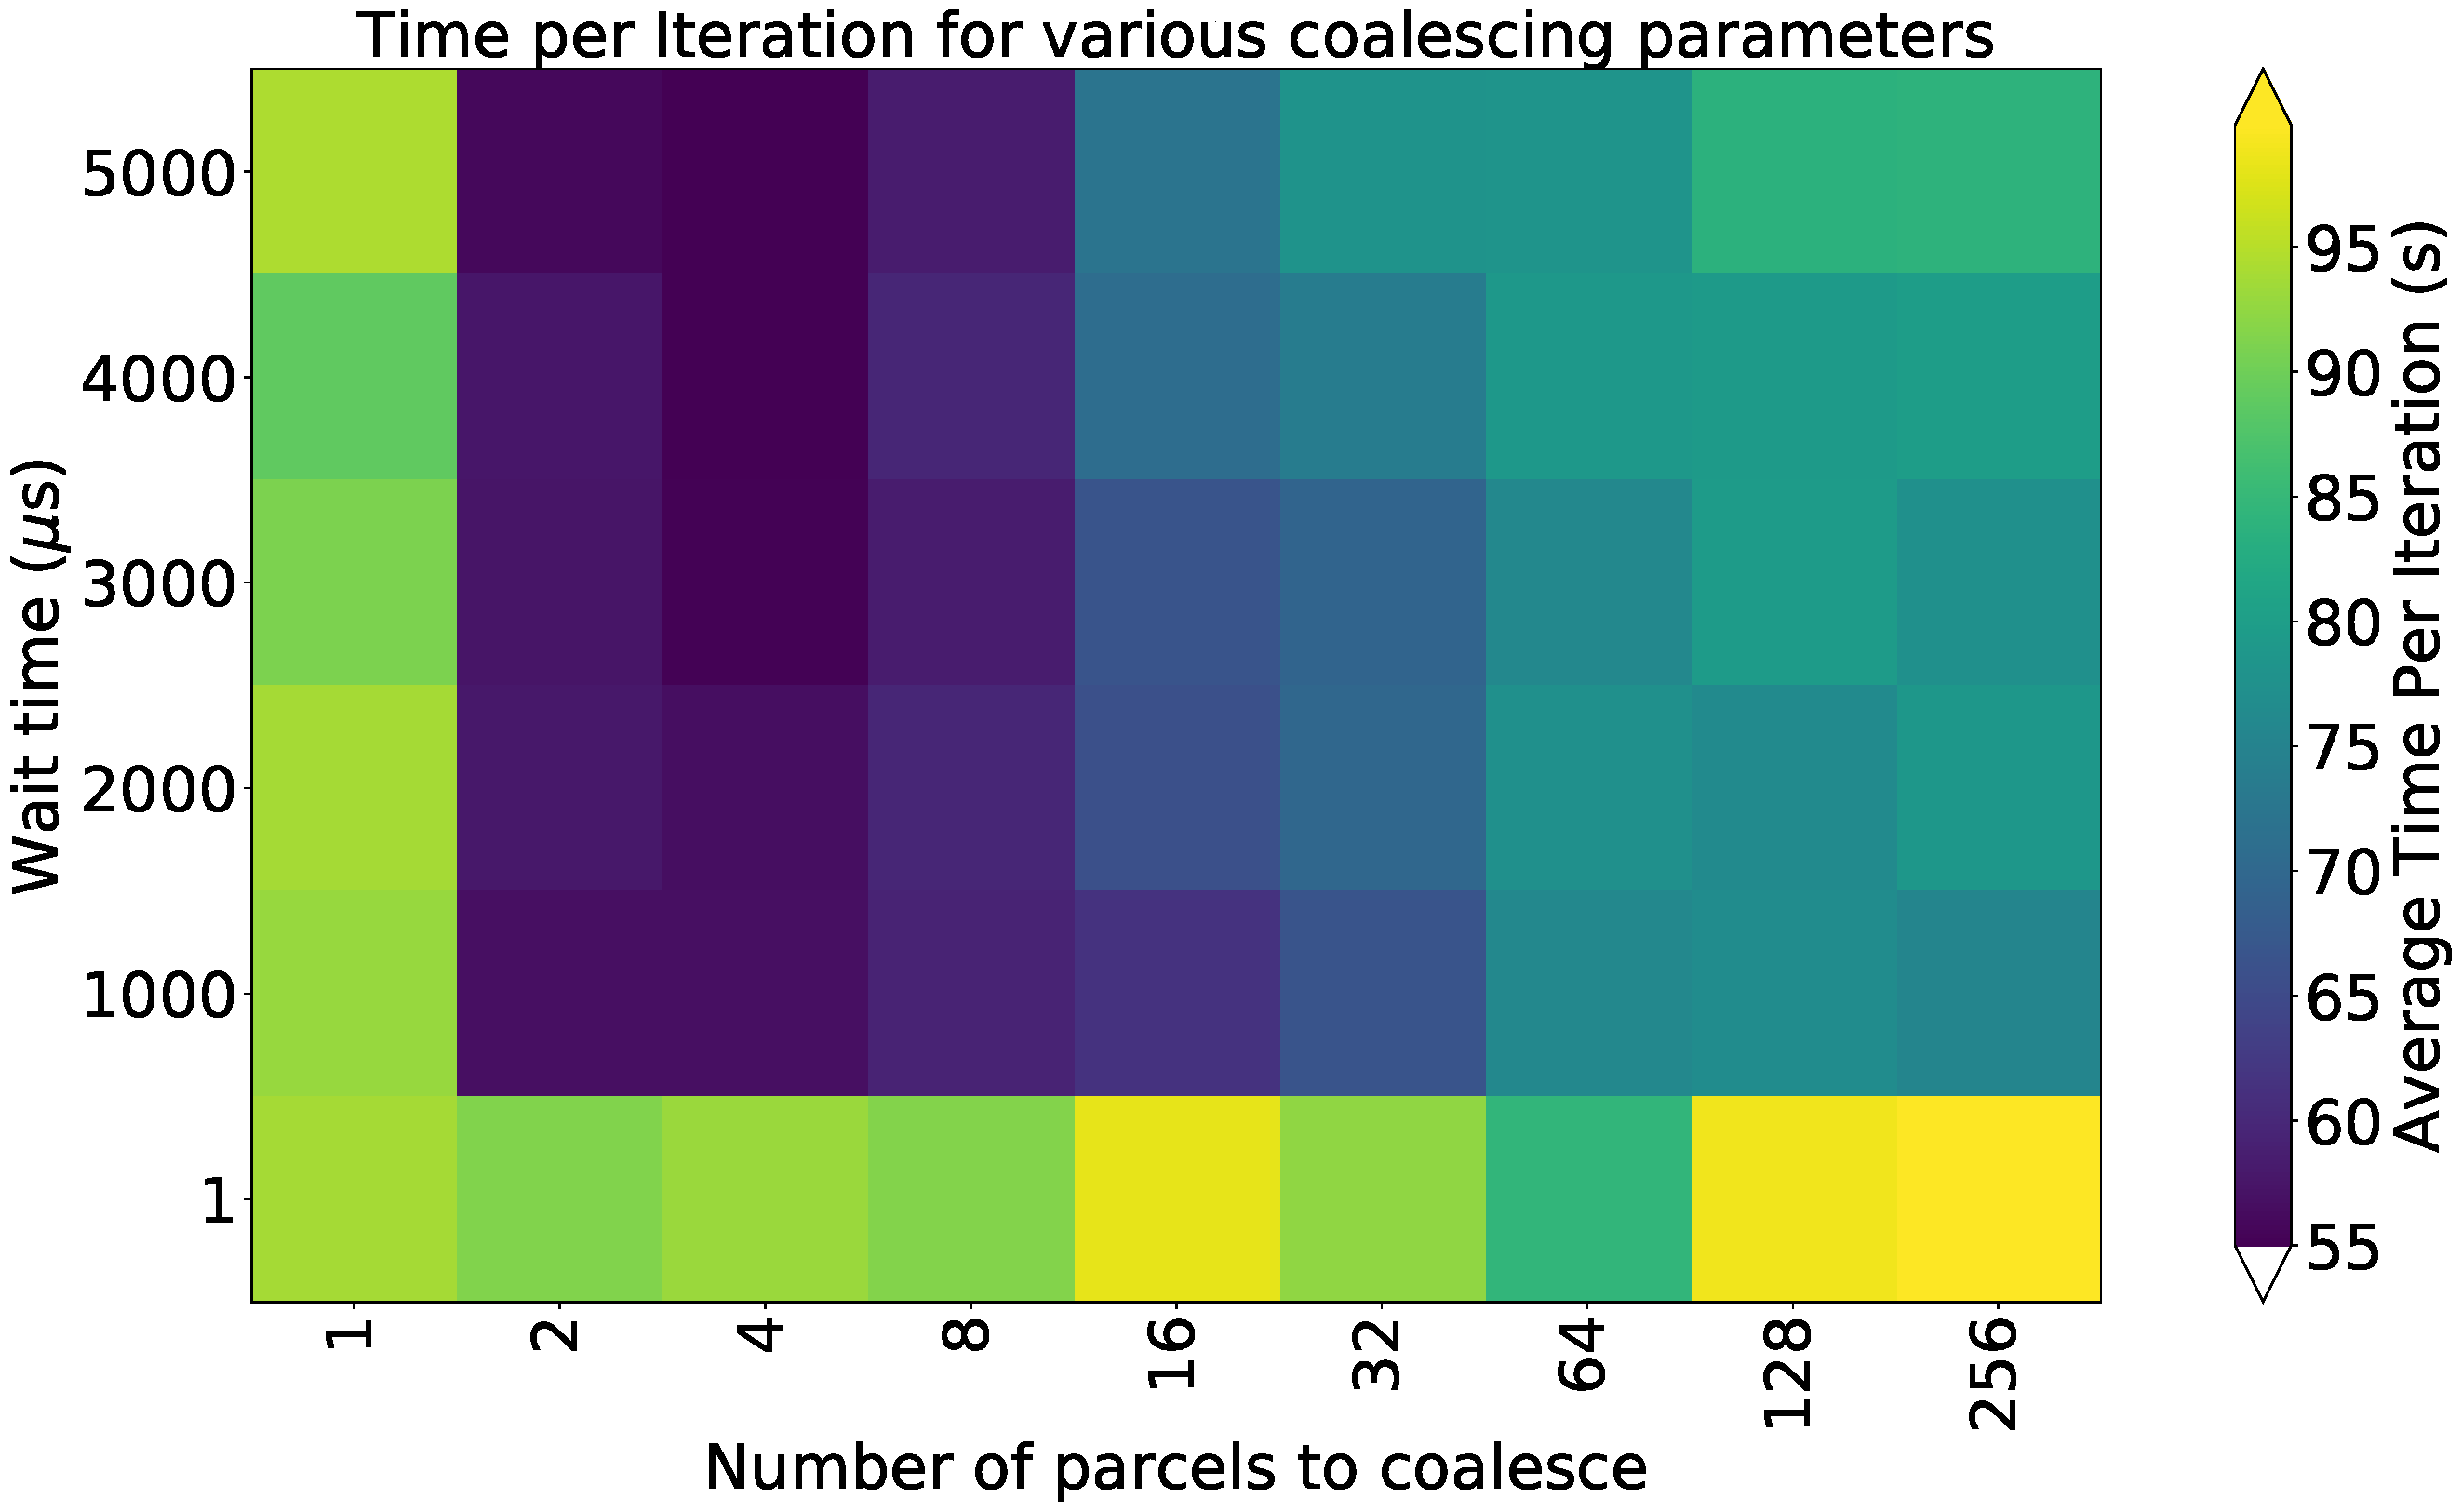
\includegraphics[width=1\linewidth]{figures/Parquet_Time_Per_Iteration.pdf}
	\caption{{Average time per iteration for various coalescing parameters.}}
	\label{figureTime-Parq}
\end{figure}
\end{frame}

\begin{frame}{Side by Side for Visual Correlation}
\begin{figure}
	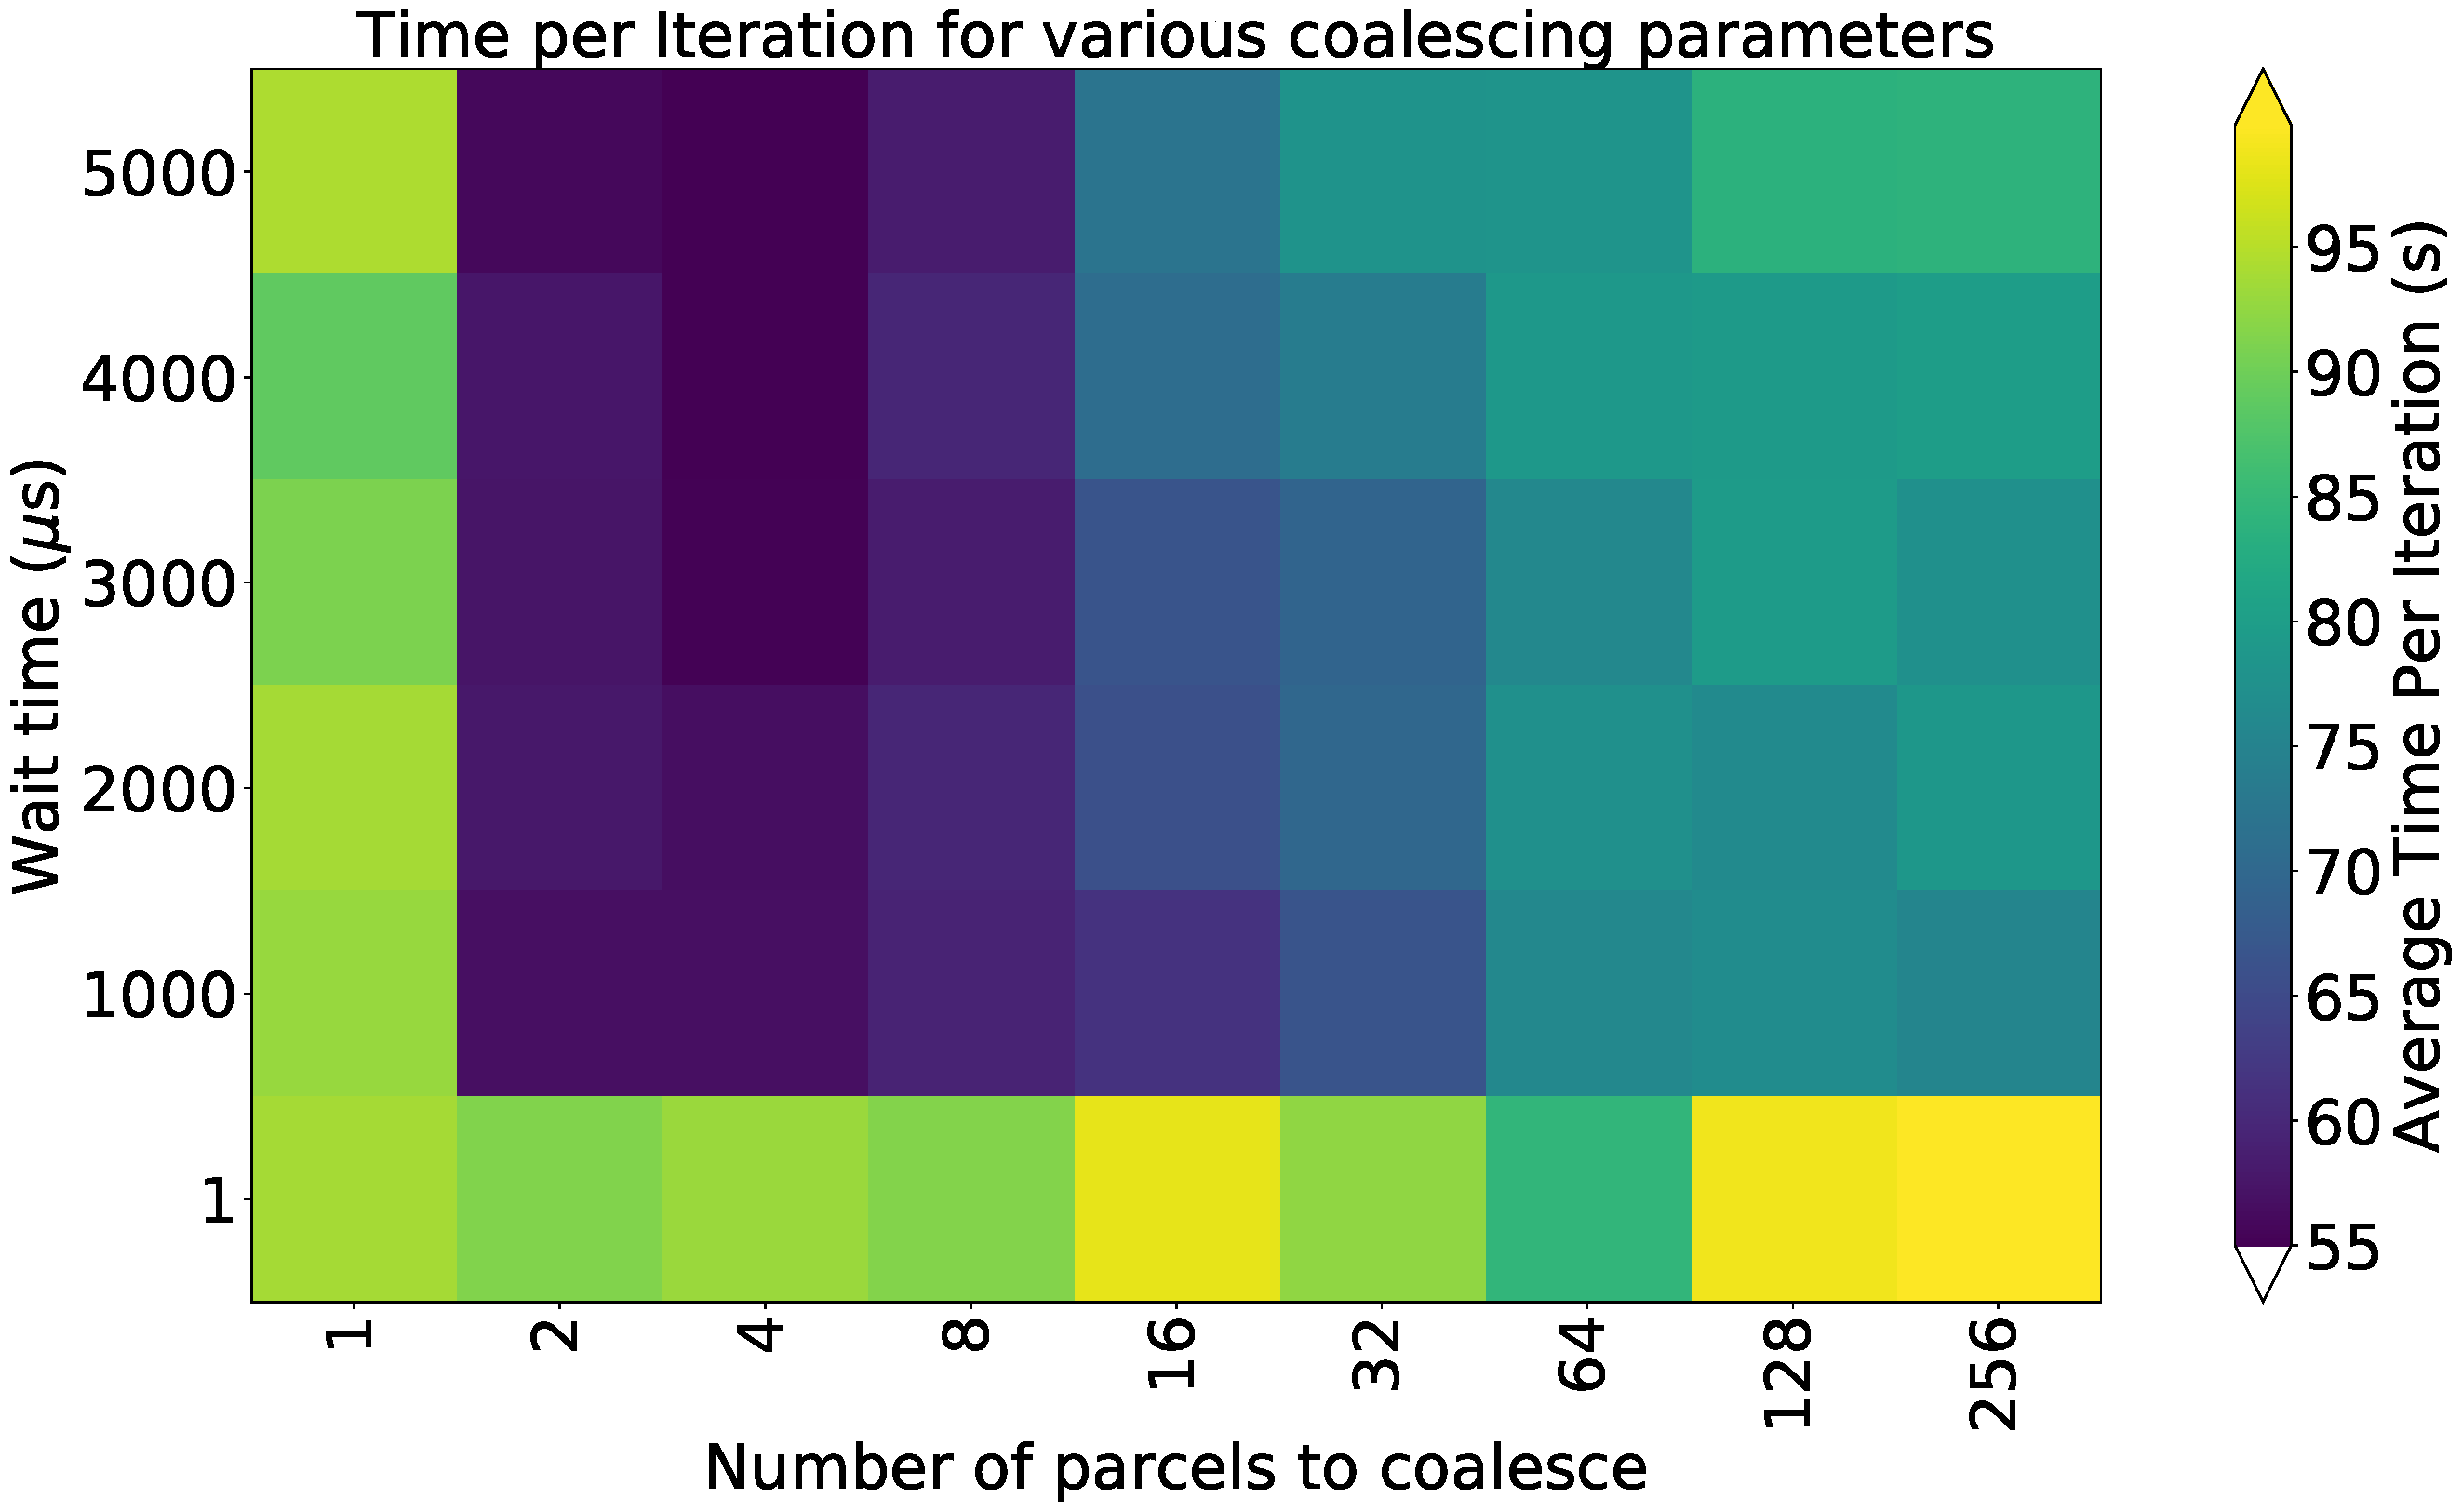
\includegraphics[width=0.52\linewidth]{figures/Parquet_Time_Per_Iteration.pdf}
	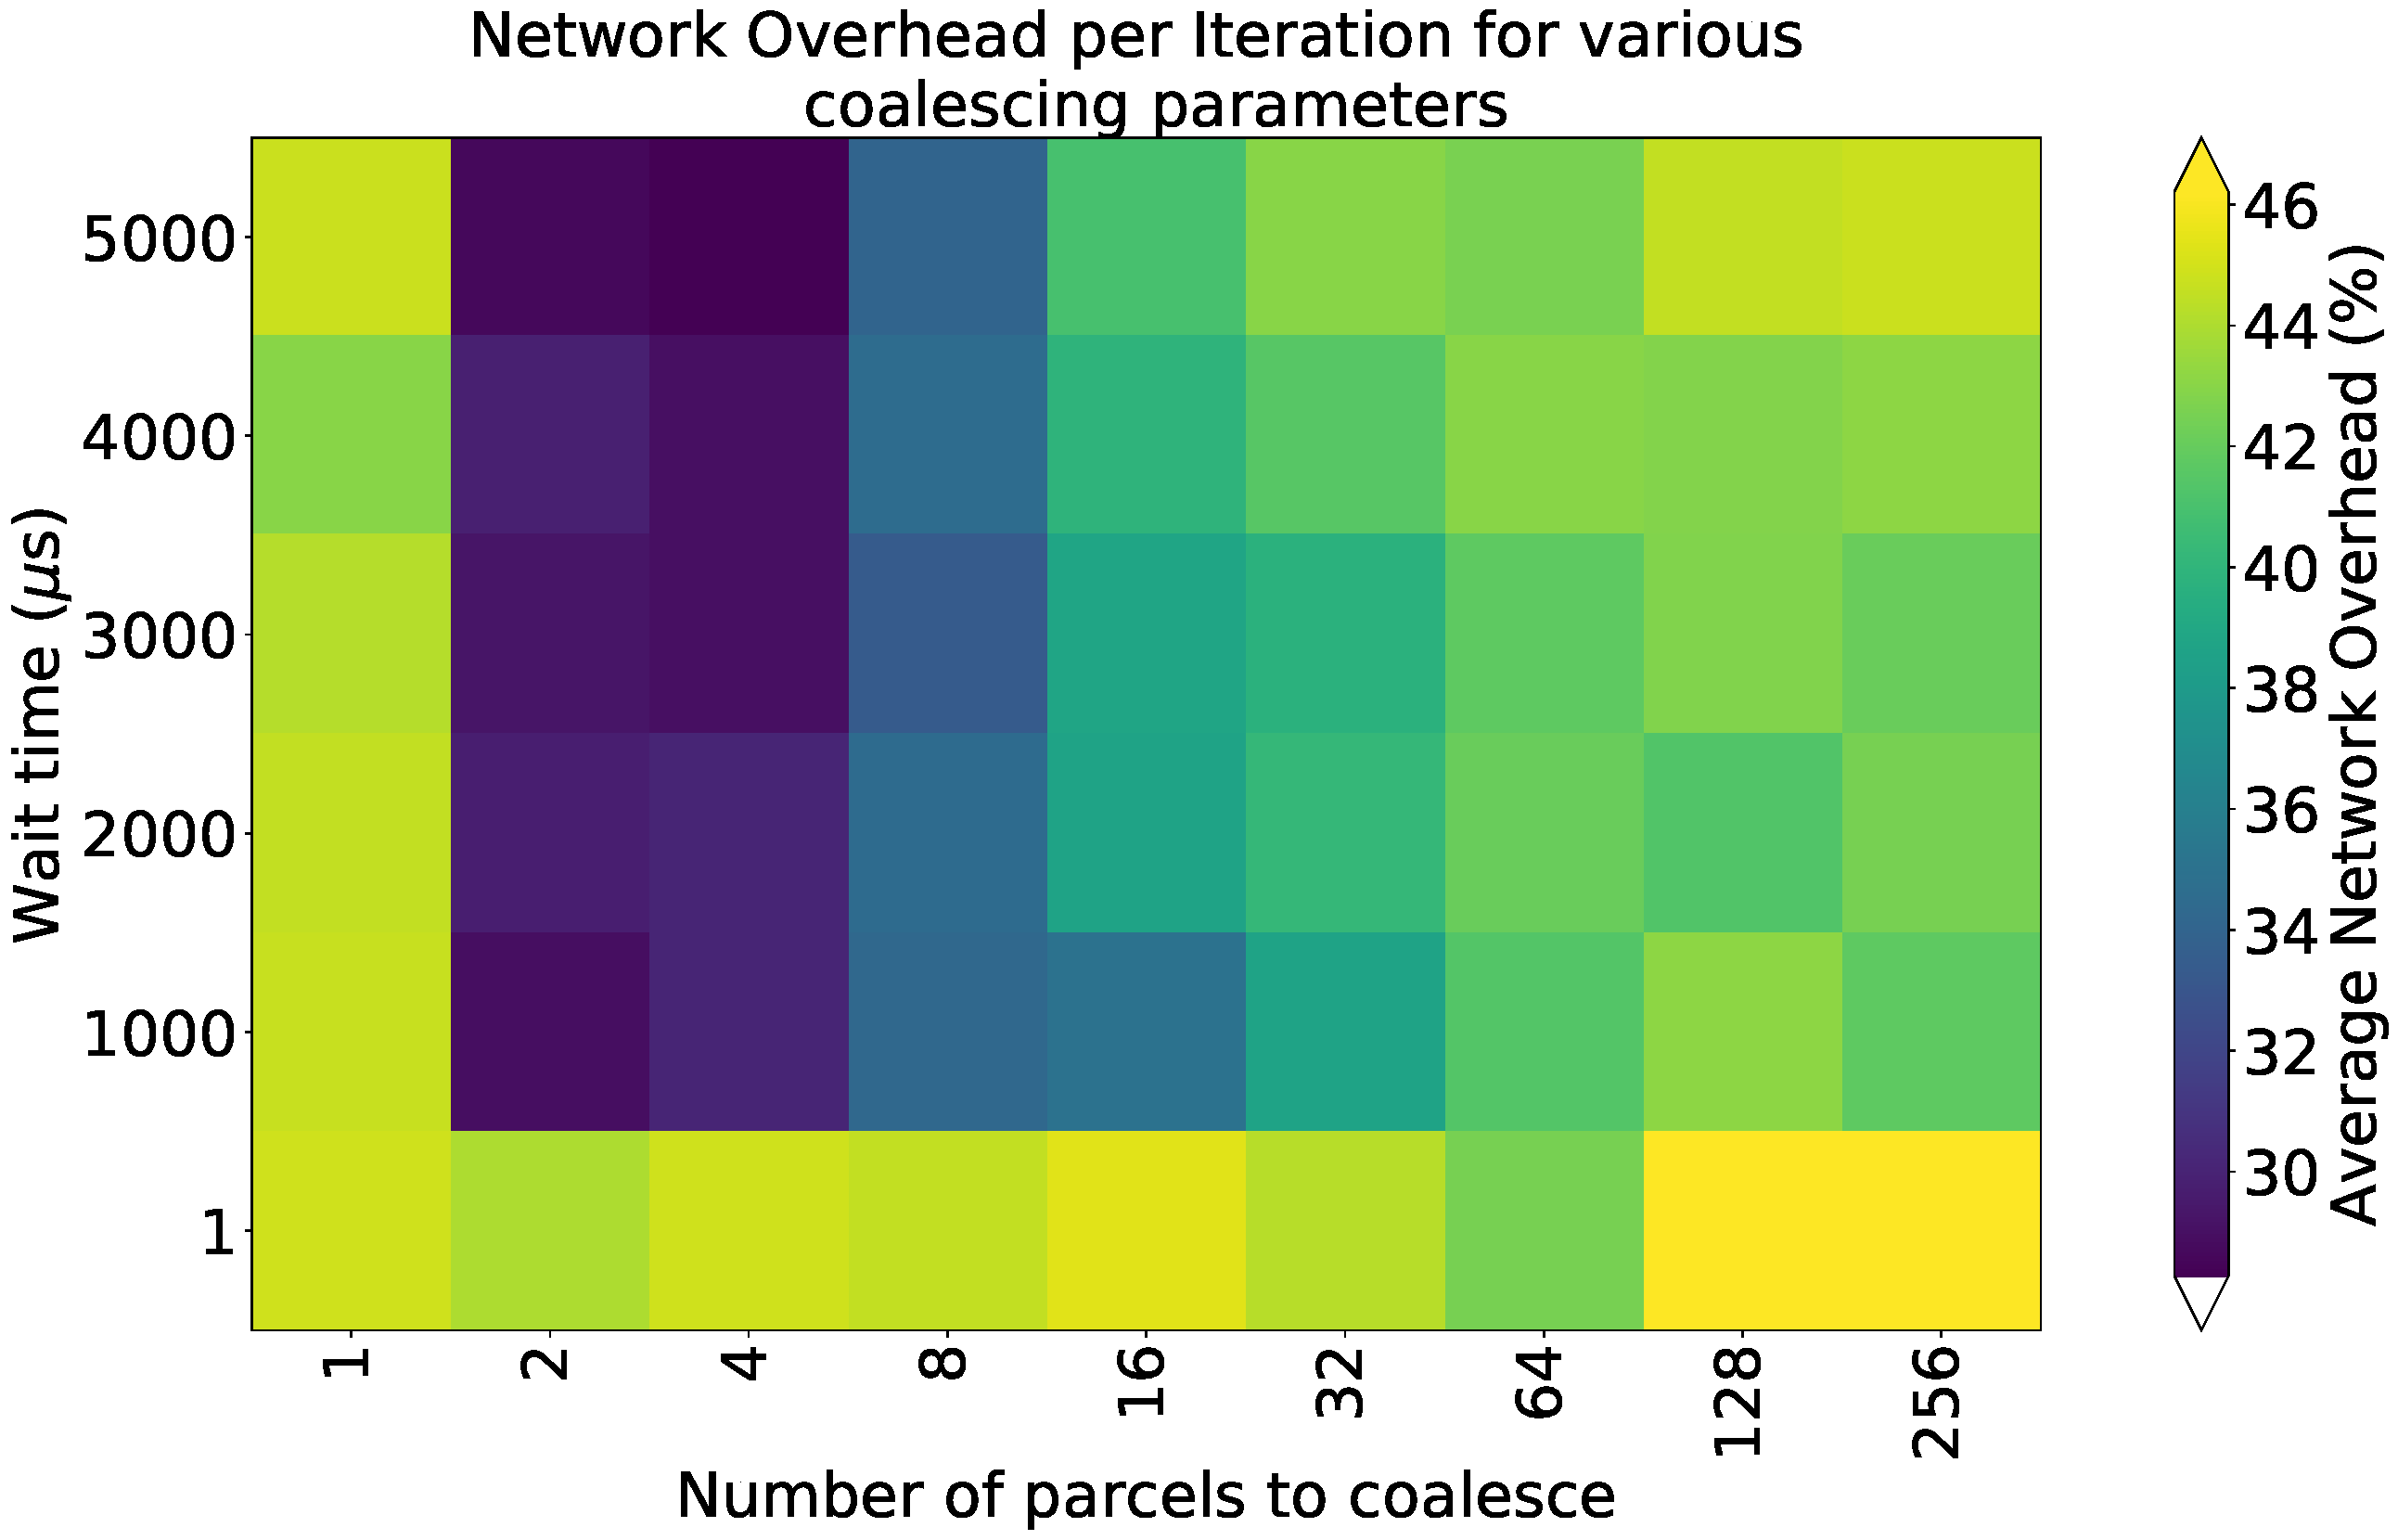
\includegraphics[width=0.52\linewidth]{figures/Parquet_Network_Overhead_Per_Iteration.pdf}
	\caption{{Average time per iteration and average Network Overhead per iteration for various coalescing parameters. }}
\end{figure}
\end{frame}

\begin{frame}{Implications}
\begin{outline}
	\1 Sub-optimal parameter selection results in drastic performance loss.
	\1 Non-availability of methods other than brute force  to ``guess" coalescing parameters signals need for adaptive methods.
	\1 Metrics identified in this research showed strong positive correlation with execution time for two different applications.
	\1 Initial results hints towards the possibility of being able to use our metrics for adaptive tuning of parcel coalescing.
\end{outline}
\end{frame}

\begin{frame}{Contributions}
The contributions  of this research so far are as follows: 
\begin{enumerate}
	\item Identification of metrics that measure instantaneous network overhead and eventually could be used in adaptive tuning of distributed applications. 
	\item Implementation of parcel coalescing in HPX and significant improvement in scientific application performance as a result. 
\end{enumerate}
\alert{Work In Progress:} \\
Utilization of identified metrics and runtime characteristics for adaptive tuning of coalescing parameters 
\end{frame}

\begin{frame}{Publications}
The research so far has resulted in the following publications: 
\begin{outline}
	\1 B. Wagle, S. Kellar, A. Serio and H. Kaiser:\textbf{ Methodology for Adaptive Active Message Coalescing in Task Based Runtime System}, 13th International Workshop on Automatic Performance Tuning (iWAPT/IPDPS-W) 2018.
	\1 B. Wagle, S. Kellar, S.X. Yang, K.M. Tam, H. Kaiser, M. Jarrell, J. Moreno: \textbf{HPX Implementation of Parquet Approximation}, SCALA 2016, Poster Session.
	\1 B. Wagle, S. Kellar, S.X. Yang, K.M. Tam, A. Serio, H. Kaiser, J. Moreno, M. Jarrell: \textbf{Parquet in the Multiscale Era} , Proceedings of Louisiana EPSCoR RII LA-SiGMA 2015 Symposium.
\end{outline}
\end{frame}

\section{Managing Scheduling Overhead}

\begin{frame}{Approaches to Managing Overheads}
\begin{outline}
	\1 Grain Size Control 
		\2 Control the size of the task being generated 
		\2 Task inlining for grain size control
	\1 Cutoff Technique
		\2 Do not create tasks beyond a certain threshold
\end{outline}	
\end{frame}

\begin{frame}{Machine Learning Applications}
\begin{outline}
	\1 Machine learning applications are starting to make more use of HPC resources
	\1 Applications tends to be iterative which provides lucrative opportunities for adaptivity
\end{outline}
\end{frame}

\begin{frame}{Experimentation on Phylanx}
\begin{outline}
	\1 Phylanx : A task based asynchronous distributed array computation toolkit 
	\1 Performance benefits of HPC systems with the ease of programming in a high level language
	\1 Python frontend to abstracts away complexities of lower level implementations (HPX)
	\1 Run NumPy code directly in Phylanx
	\1 Task graphs are generated from Python
	\1 HPX acts as the execution engine to execute the task graphs
\end{outline}
\end{frame}

\begin{frame}{Architecture of Phylanx}
\begin{figure}[!h]
	\centering
	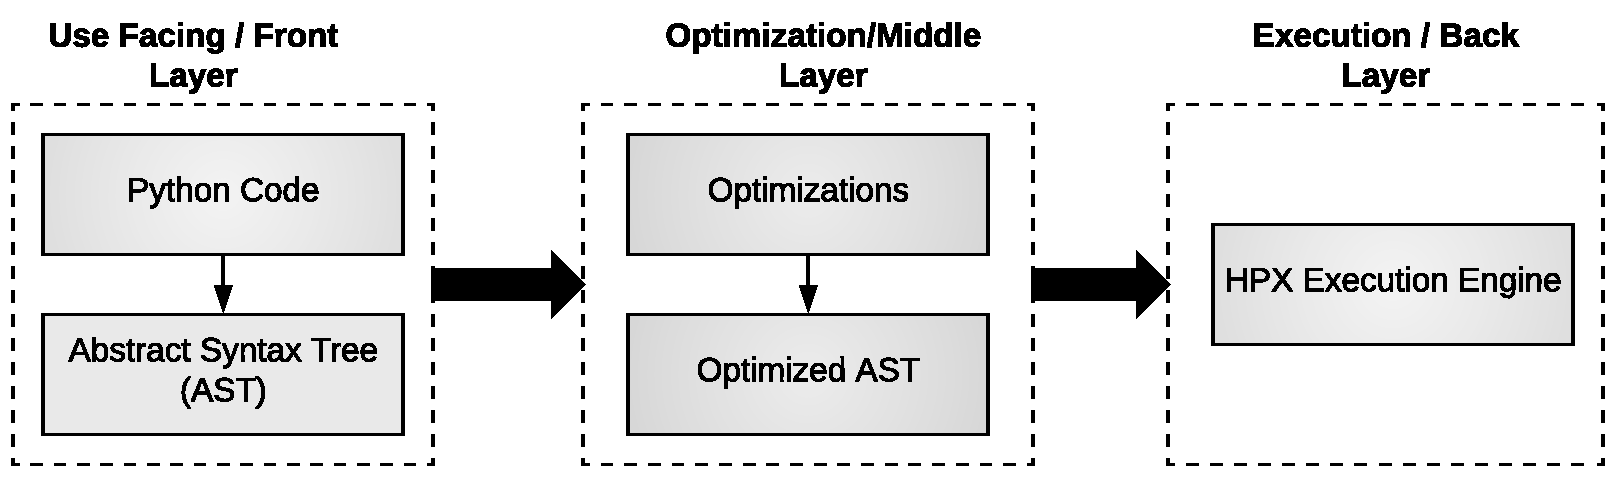
\includegraphics[width=1\linewidth]{figures/phylanx_arch.pdf}
	\caption{Architecture of Phylanx }
\end{figure}
\end{frame}

\begin{frame}{Why Phylanx}
\begin{outline}
	\1 Primitives, which are the smallest independent amount of work that can be performed
	\1 HPX executes each primitives as a task
	\1 Phylanx already has the infrastructure in place to measure the execution time and count of each primitive execution.
	\1 Phylanx supports performance counters which is vital for adaptive decision making.
\end{outline}
\end{frame}

\begin{frame}{Preliminary Assessment of Task Overheads}
\begin{outline}
	\1 Implementation of Naive Logistic Regression Algorithm 
	\1 Experimental Testbed 
		\2 Marvin Thin Compute Nodes of ROSTAM Cluster 
		\2 2x Intel Xeon E5-2450 CPU 16 Cores total 
		\2 48GB 1333 MHZ DDR3 Memory 
		\2 HPX v 1.2, Phylanx v 0.1 and  GCC 7.3 
	\1 Inlined tasks to access overheads
\end{outline}
\end{frame}

\begin{frame}{Cost of Asynchrony}
\begin{figure}
	\centering
	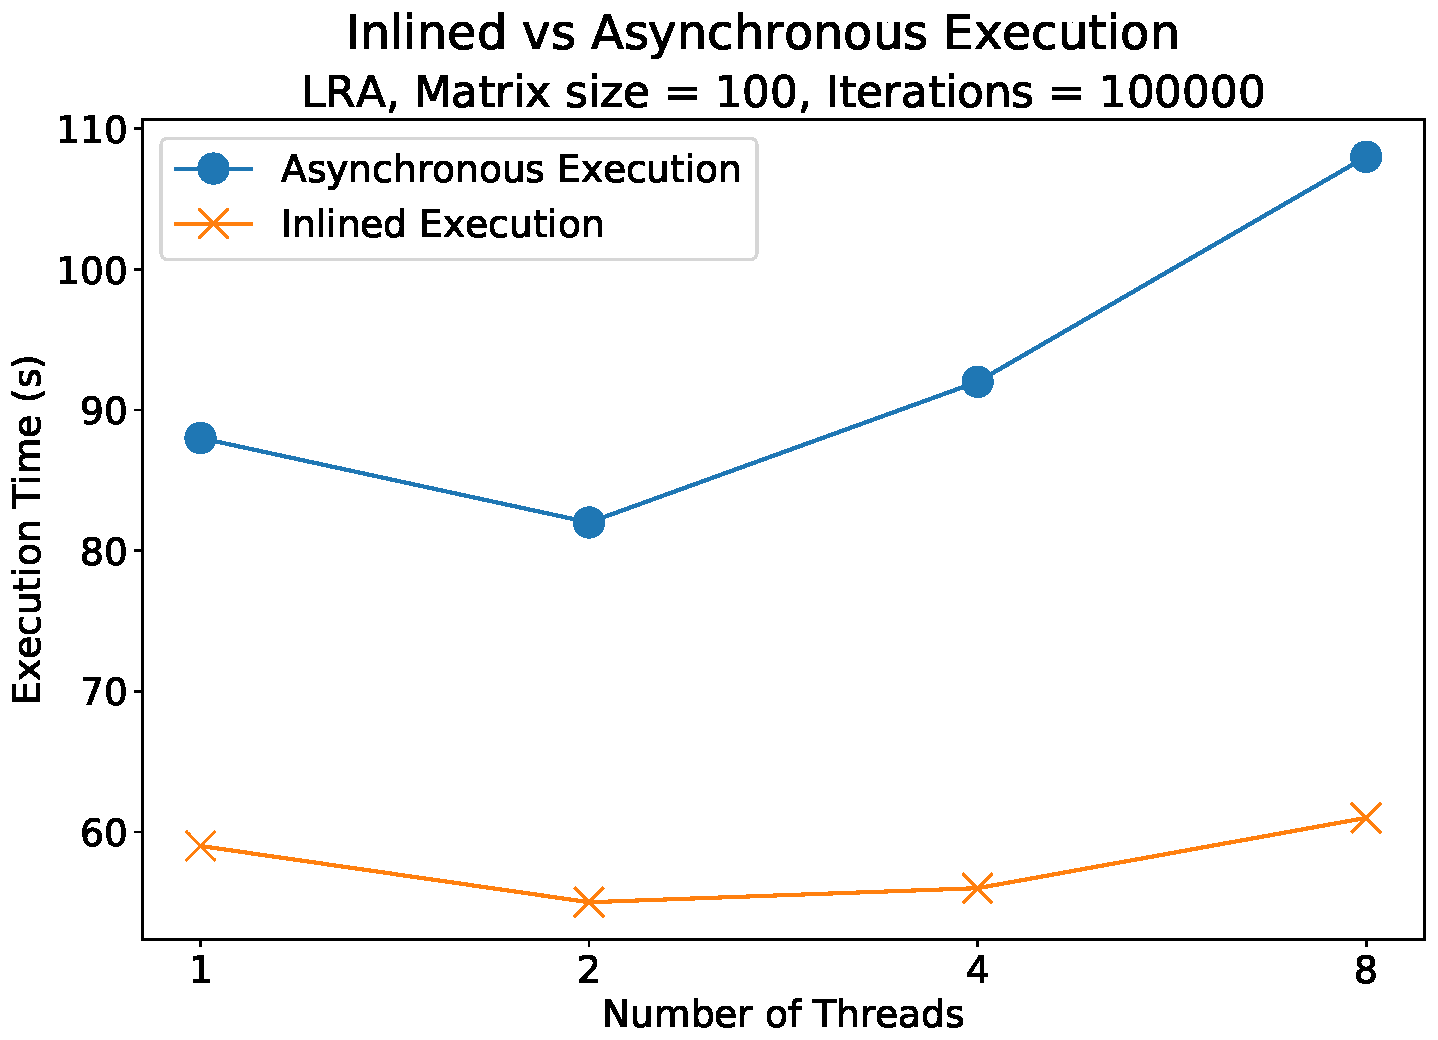
\includegraphics[width=0.8\linewidth]{figures/direct_nondir.pdf}
	\par\caption{Results of running the Logistic Regression Algorithm with custom dataset of size 100 features.}
	\label{dir_nondir}
\end{figure}
\end{frame}

\begin{frame}{Room for Improvement}
\begin{outline}
	\1 Preliminary results show  asynchronous execution resulted in slower performance compared to inlined execution for small matrix size. 
	\1 Overheads associated with task creation and scheduling play a role in slower execution time. 
	\1 Overheads vary with problem size or the underlying system.
	\1 Such complexities warrant the need for adaptive approach to overhead reduction.
\end{outline}
\end{frame}

\begin{frame}{Related Work}
\begin{outline}
	\1 Mohr, introduced lazy task creation methods, where tasks are inlined but enough information is saved such that if need arises, could be executed asynchronously. 
	\1 With regards to OpenMP tasks, Alejandro Duran  employed  adaptive cut-off technique by using information collected at runtime.
	\1 In a previous study on HPX, Patricia Grubel, used performance counters for dynamically tuning grain size of 1d-stencil application..  
	\1 In Charm++, ParSSSE framework initially generates tasks to saturate all cores with work. The framework then decides whether to parallelize subsequent tasks or not based on execution time of the tasks compared to the overhead associated with its creation. 
\end{outline}
\end{frame}

\section{Proposed Study}

\begin{frame}{Future Work}
\begin{outline}
	\1 Implement advanced adaptive parcel coalescing in HPX using the matrices identified,
	\1 Analyze task scheduling and execution overheads in context of Phylanx, and
	\1 Implement adaptive techniques for reduction of scheduling and execution overhead.
\end{outline}
\end{frame}

\begin{frame}{Timeline}
\begin{outline}
	\1 Adaptive Coalescing (3 months)
		\2 Parcel Coalescing APEX Policy in HPX 
		\2 Identification of appropriate spot / criteria for APEX policy trigger
		\2 Testing with Parquet and one more application, preferably Octotiger.
	\1 Identification of appropriate strategy/methodology for reducing overheads in Phylanx/HPX. (4 months)
	\1 Adaptive Method for reducing overheads in Phylanx/HPX. (5 Months)
	\1 Estimated completion of proposed work : 1 Year
\end{outline}
\end{frame}

\begin{frame}{Support}
 This work was partly funded by the NSF EPSCoR LA-SiGMA project under award \#EPS-1003897 ,the NSF STORM project under the award \#ACI-1339782 and NSF Phylanx project award \#1737785. Any opinions, findings, and conclusions or recommendations expressed in this material are those of the authors and do not necessarily reflect the views of the National Science Foundation.
\end{frame}

\begin{frame}[standout]
  Questions?
\end{frame}

\appendix

\begin{frame}[fragile]{Backup slides}
The following slides are backup slides. 
\end{frame}

\begin{frame}{Parquet Network Overhead}
\begin{figure}
	\centering
	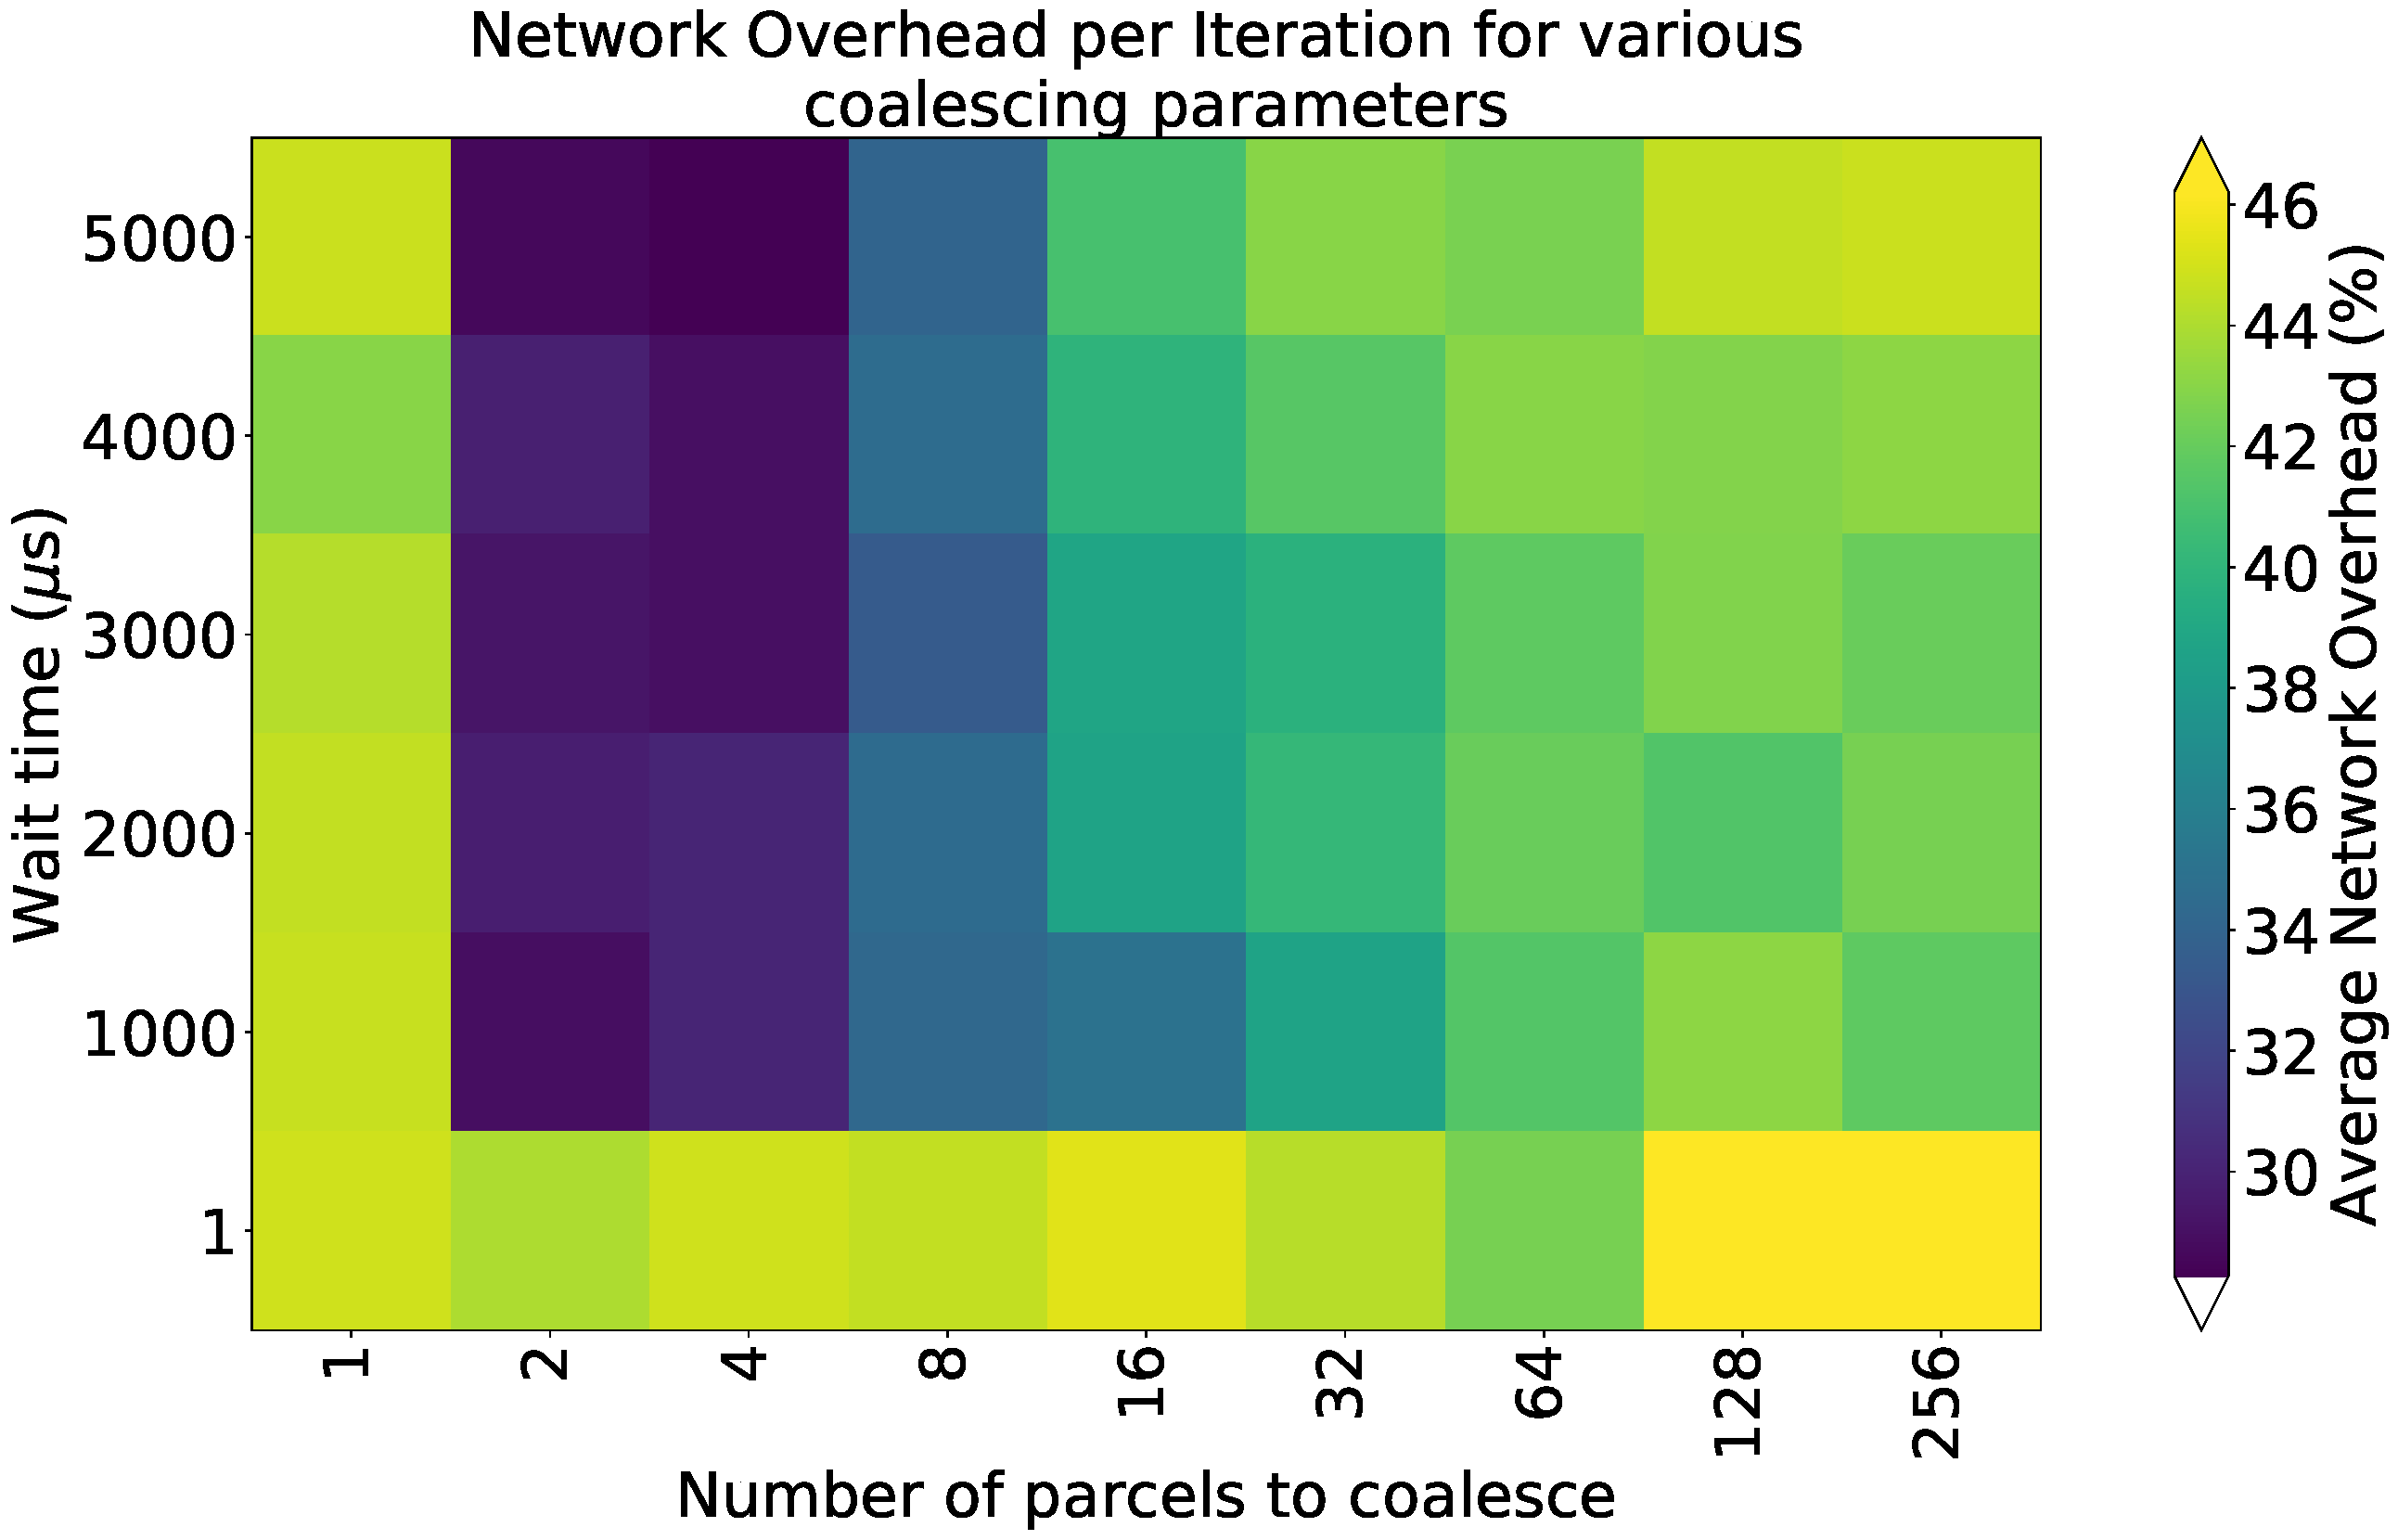
\includegraphics[width=1\linewidth]{figures/Parquet_Network_Overhead_Per_Iteration.pdf}
	\caption{{Average Network Overhead per iteration for various coalescing parameters.}}
	\label{figureTime-Parq}
\end{figure}
\end{frame}


\end{document}
